\documentclass[twoside]{book}

% Packages required by doxygen
\usepackage{fixltx2e}
\usepackage{calc}
\usepackage{doxygen}
\usepackage[export]{adjustbox} % also loads graphicx
\usepackage{graphicx}
\usepackage[utf8]{inputenc}
\usepackage{makeidx}
\usepackage{multicol}
\usepackage{multirow}
\PassOptionsToPackage{warn}{textcomp}
\usepackage{textcomp}
\usepackage[nointegrals]{wasysym}
\usepackage[table]{xcolor}

% Font selection
\usepackage[T1]{fontenc}
\usepackage[scaled=.90]{helvet}
\usepackage{courier}
\usepackage{amssymb}
\usepackage{sectsty}
\renewcommand{\familydefault}{\sfdefault}
\allsectionsfont{%
  \fontseries{bc}\selectfont%
  \color{darkgray}%
}
\renewcommand{\DoxyLabelFont}{%
  \fontseries{bc}\selectfont%
  \color{darkgray}%
}
\newcommand{\+}{\discretionary{\mbox{\scriptsize$\hookleftarrow$}}{}{}}

% Page & text layout
\usepackage{geometry}
\geometry{%
  a4paper,%
  top=2.5cm,%
  bottom=2.5cm,%
  left=2.5cm,%
  right=2.5cm%
}
\tolerance=750
\hfuzz=15pt
\hbadness=750
\setlength{\emergencystretch}{15pt}
\setlength{\parindent}{0cm}
\setlength{\parskip}{3ex plus 2ex minus 2ex}
\makeatletter
\renewcommand{\paragraph}{%
  \@startsection{paragraph}{4}{0ex}{-1.0ex}{1.0ex}{%
    \normalfont\normalsize\bfseries\SS@parafont%
  }%
}
\renewcommand{\subparagraph}{%
  \@startsection{subparagraph}{5}{0ex}{-1.0ex}{1.0ex}{%
    \normalfont\normalsize\bfseries\SS@subparafont%
  }%
}
\makeatother

% Headers & footers
\usepackage{fancyhdr}
\pagestyle{fancyplain}
\fancyhead[LE]{\fancyplain{}{\bfseries\thepage}}
\fancyhead[CE]{\fancyplain{}{}}
\fancyhead[RE]{\fancyplain{}{\bfseries\leftmark}}
\fancyhead[LO]{\fancyplain{}{\bfseries\rightmark}}
\fancyhead[CO]{\fancyplain{}{}}
\fancyhead[RO]{\fancyplain{}{\bfseries\thepage}}
\fancyfoot[LE]{\fancyplain{}{}}
\fancyfoot[CE]{\fancyplain{}{}}
\fancyfoot[RE]{\fancyplain{}{\bfseries\scriptsize Generated by Doxygen }}
\fancyfoot[LO]{\fancyplain{}{\bfseries\scriptsize Generated by Doxygen }}
\fancyfoot[CO]{\fancyplain{}{}}
\fancyfoot[RO]{\fancyplain{}{}}
\renewcommand{\footrulewidth}{0.4pt}
\renewcommand{\chaptermark}[1]{%
  \markboth{#1}{}%
}
\renewcommand{\sectionmark}[1]{%
  \markright{\thesection\ #1}%
}

% Indices & bibliography
\usepackage{natbib}
\usepackage[titles]{tocloft}
\setcounter{tocdepth}{3}
\setcounter{secnumdepth}{5}
\makeindex

% Hyperlinks (required, but should be loaded last)
\usepackage{ifpdf}
\ifpdf
  \usepackage[pdftex,pagebackref=true]{hyperref}
\else
  \usepackage[ps2pdf,pagebackref=true]{hyperref}
\fi
\hypersetup{%
  colorlinks=true,%
  linkcolor=blue,%
  citecolor=blue,%
  unicode%
}

% Custom commands
\newcommand{\clearemptydoublepage}{%
  \newpage{\pagestyle{empty}\cleardoublepage}%
}

\usepackage{caption}
\captionsetup{labelsep=space,justification=centering,font={bf},singlelinecheck=off,skip=4pt,position=top}

%===== C O N T E N T S =====

\begin{document}

% Titlepage & ToC
\hypersetup{pageanchor=false,
             bookmarksnumbered=true,
             pdfencoding=unicode
            }
\pagenumbering{roman}
\begin{titlepage}
\vspace*{7cm}
\begin{center}%
{\Large Prac }\\
\vspace*{1cm}
{\large Generated by Doxygen 1.8.11}\\
\end{center}
\end{titlepage}
\clearemptydoublepage
\tableofcontents
\clearemptydoublepage
\pagenumbering{arabic}
\hypersetup{pageanchor=true}

%--- Begin generated contents ---
\chapter{Hierarchical Index}
\section{Class Hierarchy}
This inheritance list is sorted roughly, but not completely, alphabetically\+:\begin{DoxyCompactList}
\item \contentsline{section}{Album\+\_\+}{\pageref{struct_album__}}{}
\item \contentsline{section}{Catalog\+\_\+\+:\+:Album\+Entity}{\pageref{struct_catalog___1_1_album_entity}}{}
\item \contentsline{section}{Author\+\_\+}{\pageref{struct_author__}}{}
\item \contentsline{section}{Catalog\+\_\+\+:\+:Author\+Entity}{\pageref{struct_catalog___1_1_author_entity}}{}
\item \contentsline{section}{Catalog\+\_\+}{\pageref{class_catalog__}}{}
\item \contentsline{section}{Catalog\+Loader}{\pageref{class_catalog_loader}}{}
\item \contentsline{section}{Event\+\_\+}{\pageref{struct_event__}}{}
\begin{DoxyCompactList}
\item \contentsline{section}{End\+Of\+Song\+Event\+\_\+}{\pageref{struct_end_of_song_event__}}{}
\item \contentsline{section}{Query\+Event\+\_\+}{\pageref{struct_query_event__}}{}
\end{DoxyCompactList}
\item \contentsline{section}{Radio\+Program\+Simulator\+\_\+\+:\+:Event\+Comparator}{\pageref{struct_radio_program_simulator___1_1_event_comparator}}{}
\item \contentsline{section}{File\+Utils}{\pageref{class_file_utils}}{}
\item \contentsline{section}{Genre\+\_\+}{\pageref{struct_genre__}}{}
\item \contentsline{section}{Catalog\+\_\+\+:\+:Genre\+Entity}{\pageref{struct_catalog___1_1_genre_entity}}{}
\item \contentsline{section}{Play\+\_\+}{\pageref{struct_play__}}{}
\item Q\+Dialog\begin{DoxyCompactList}
\item \contentsline{section}{Album\+Describer}{\pageref{class_album_describer}}{}
\item \contentsline{section}{Author\+Describer}{\pageref{class_author_describer}}{}
\item \contentsline{section}{Genre\+Discriber}{\pageref{class_genre_discriber}}{}
\item \contentsline{section}{Song\+Describer}{\pageref{class_song_describer}}{}
\end{DoxyCompactList}
\item Q\+Main\+Window\begin{DoxyCompactList}
\item \contentsline{section}{Main\+Window}{\pageref{class_main_window}}{}
\end{DoxyCompactList}
\item \contentsline{section}{Query\+\_\+}{\pageref{struct_query__}}{}
\begin{DoxyCompactList}
\item \contentsline{section}{Album\+Query\+\_\+}{\pageref{struct_album_query__}}{}
\item \contentsline{section}{Author\+Query\+\_\+}{\pageref{struct_author_query__}}{}
\item \contentsline{section}{Song\+Query\+\_\+}{\pageref{struct_song_query__}}{}
\end{DoxyCompactList}
\item Q\+Widget\begin{DoxyCompactList}
\item \contentsline{section}{Storage\+Form}{\pageref{class_storage_form}}{}
\item \contentsline{section}{Timetable\+Editor\+Form}{\pageref{class_timetable_editor_form}}{}
\end{DoxyCompactList}
\item \contentsline{section}{Radio\+Program\+\_\+}{\pageref{class_radio_program__}}{}
\begin{DoxyCompactList}
\item \contentsline{section}{Hit\+Parad\+Program\+\_\+}{\pageref{class_hit_parad_program__}}{}
\item \contentsline{section}{Requests\+Program\+\_\+}{\pageref{class_requests_program__}}{}
\end{DoxyCompactList}
\item \contentsline{section}{Radio\+Program\+Simulator\+\_\+}{\pageref{class_radio_program_simulator__}}{}
\begin{DoxyCompactList}
\item \contentsline{section}{Hit\+Parad\+Program\+Simulator\+\_\+}{\pageref{class_hit_parad_program_simulator__}}{}
\item \contentsline{section}{Requests\+Program\+Simulator\+\_\+}{\pageref{class_requests_program_simulator__}}{}
\end{DoxyCompactList}
\item \contentsline{section}{Requests\+Generator}{\pageref{class_requests_generator}}{}
\item \contentsline{section}{Royal\+Manager}{\pageref{class_royal_manager}}{}
\item \contentsline{section}{Simulator\+\_\+}{\pageref{class_simulator__}}{}
\item \contentsline{section}{Song\+\_\+}{\pageref{struct_song__}}{}
\item \contentsline{section}{Catalog\+\_\+\+:\+:Song\+Entity}{\pageref{struct_catalog___1_1_song_entity}}{}
\item \contentsline{section}{Statistics\+\_\+}{\pageref{class_statistics__}}{}
\item \contentsline{section}{Statistics\+Event\+\_\+}{\pageref{struct_statistics_event__}}{}
\begin{DoxyCompactList}
\item \contentsline{section}{Play\+Event\+\_\+}{\pageref{struct_play_event__}}{}
\item \contentsline{section}{Statistics\+Query\+Event\+\_\+}{\pageref{struct_statistics_query_event__}}{}
\end{DoxyCompactList}
\item \contentsline{section}{Timetable\+Loader}{\pageref{class_timetable_loader}}{}
\end{DoxyCompactList}

\chapter{Class Index}
\section{Class List}
Here are the classes, structs, unions and interfaces with brief descriptions\+:\begin{DoxyCompactList}
\item\contentsline{section}{\hyperlink{struct_album__}{Album\+\_\+} }{\pageref{struct_album__}}{}
\item\contentsline{section}{\hyperlink{class_album_describer}{Album\+Describer} }{\pageref{class_album_describer}}{}
\item\contentsline{section}{\hyperlink{struct_catalog___1_1_album_entity}{Catalog\+\_\+\+::\+Album\+Entity} }{\pageref{struct_catalog___1_1_album_entity}}{}
\item\contentsline{section}{\hyperlink{struct_album_query__}{Album\+Query\+\_\+} }{\pageref{struct_album_query__}}{}
\item\contentsline{section}{\hyperlink{struct_author__}{Author\+\_\+} }{\pageref{struct_author__}}{}
\item\contentsline{section}{\hyperlink{class_author_describer}{Author\+Describer} }{\pageref{class_author_describer}}{}
\item\contentsline{section}{\hyperlink{struct_catalog___1_1_author_entity}{Catalog\+\_\+\+::\+Author\+Entity} }{\pageref{struct_catalog___1_1_author_entity}}{}
\item\contentsline{section}{\hyperlink{struct_author_query__}{Author\+Query\+\_\+} }{\pageref{struct_author_query__}}{}
\item\contentsline{section}{\hyperlink{class_catalog__}{Catalog\+\_\+} }{\pageref{class_catalog__}}{}
\item\contentsline{section}{\hyperlink{class_catalog_loader}{Catalog\+Loader} }{\pageref{class_catalog_loader}}{}
\item\contentsline{section}{\hyperlink{struct_end_of_song_event__}{End\+Of\+Song\+Event\+\_\+} }{\pageref{struct_end_of_song_event__}}{}
\item\contentsline{section}{\hyperlink{struct_event__}{Event\+\_\+} }{\pageref{struct_event__}}{}
\item\contentsline{section}{\hyperlink{struct_radio_program_simulator___1_1_event_comparator}{Radio\+Program\+Simulator\+\_\+\+::\+Event\+Comparator} }{\pageref{struct_radio_program_simulator___1_1_event_comparator}}{}
\item\contentsline{section}{\hyperlink{class_file_utils}{File\+Utils} }{\pageref{class_file_utils}}{}
\item\contentsline{section}{\hyperlink{struct_genre__}{Genre\+\_\+} }{\pageref{struct_genre__}}{}
\item\contentsline{section}{\hyperlink{class_genre_discriber}{Genre\+Discriber} }{\pageref{class_genre_discriber}}{}
\item\contentsline{section}{\hyperlink{struct_catalog___1_1_genre_entity}{Catalog\+\_\+\+::\+Genre\+Entity} }{\pageref{struct_catalog___1_1_genre_entity}}{}
\item\contentsline{section}{\hyperlink{class_hit_parad_program__}{Hit\+Parad\+Program\+\_\+} }{\pageref{class_hit_parad_program__}}{}
\item\contentsline{section}{\hyperlink{class_hit_parad_program_simulator__}{Hit\+Parad\+Program\+Simulator\+\_\+} }{\pageref{class_hit_parad_program_simulator__}}{}
\item\contentsline{section}{\hyperlink{class_main_window}{Main\+Window} }{\pageref{class_main_window}}{}
\item\contentsline{section}{\hyperlink{struct_play__}{Play\+\_\+} }{\pageref{struct_play__}}{}
\item\contentsline{section}{\hyperlink{struct_play_event__}{Play\+Event\+\_\+} }{\pageref{struct_play_event__}}{}
\item\contentsline{section}{\hyperlink{struct_query__}{Query\+\_\+} }{\pageref{struct_query__}}{}
\item\contentsline{section}{\hyperlink{struct_query_event__}{Query\+Event\+\_\+} }{\pageref{struct_query_event__}}{}
\item\contentsline{section}{\hyperlink{class_radio_program__}{Radio\+Program\+\_\+} }{\pageref{class_radio_program__}}{}
\item\contentsline{section}{\hyperlink{class_radio_program_simulator__}{Radio\+Program\+Simulator\+\_\+} }{\pageref{class_radio_program_simulator__}}{}
\item\contentsline{section}{\hyperlink{class_requests_generator}{Requests\+Generator} }{\pageref{class_requests_generator}}{}
\item\contentsline{section}{\hyperlink{class_requests_program__}{Requests\+Program\+\_\+} }{\pageref{class_requests_program__}}{}
\item\contentsline{section}{\hyperlink{class_requests_program_simulator__}{Requests\+Program\+Simulator\+\_\+} }{\pageref{class_requests_program_simulator__}}{}
\item\contentsline{section}{\hyperlink{class_royal_manager}{Royal\+Manager} }{\pageref{class_royal_manager}}{}
\item\contentsline{section}{\hyperlink{class_simulator__}{Simulator\+\_\+} }{\pageref{class_simulator__}}{}
\item\contentsline{section}{\hyperlink{struct_song__}{Song\+\_\+} }{\pageref{struct_song__}}{}
\item\contentsline{section}{\hyperlink{class_song_describer}{Song\+Describer} }{\pageref{class_song_describer}}{}
\item\contentsline{section}{\hyperlink{struct_catalog___1_1_song_entity}{Catalog\+\_\+\+::\+Song\+Entity} }{\pageref{struct_catalog___1_1_song_entity}}{}
\item\contentsline{section}{\hyperlink{struct_song_query__}{Song\+Query\+\_\+} }{\pageref{struct_song_query__}}{}
\item\contentsline{section}{\hyperlink{class_statistics__}{Statistics\+\_\+} }{\pageref{class_statistics__}}{}
\item\contentsline{section}{\hyperlink{struct_statistics_event__}{Statistics\+Event\+\_\+} }{\pageref{struct_statistics_event__}}{}
\item\contentsline{section}{\hyperlink{struct_statistics_query_event__}{Statistics\+Query\+Event\+\_\+} }{\pageref{struct_statistics_query_event__}}{}
\item\contentsline{section}{\hyperlink{class_storage_form}{Storage\+Form} }{\pageref{class_storage_form}}{}
\item\contentsline{section}{\hyperlink{class_timetable_editor_form}{Timetable\+Editor\+Form} }{\pageref{class_timetable_editor_form}}{}
\item\contentsline{section}{\hyperlink{class_timetable_loader}{Timetable\+Loader} }{\pageref{class_timetable_loader}}{}
\end{DoxyCompactList}

\chapter{Class Documentation}
\hypertarget{struct_album__}{}\section{Album\+\_\+ Struct Reference}
\label{struct_album__}\index{Album\+\_\+@{Album\+\_\+}}
\subsection*{Public Member Functions}
\begin{DoxyCompactItemize}
\item 
void {\bfseries describe} (std\+::ostream \&stream)\hypertarget{struct_album___a9cdd04dd67fd6bb92c7fb44d42f89757}{}\label{struct_album___a9cdd04dd67fd6bb92c7fb44d42f89757}

\item 
std\+::string {\bfseries processed\+Name} ()\hypertarget{struct_album___a946bb4b842ab1aedc5f9b9bc9bcc0062}{}\label{struct_album___a946bb4b842ab1aedc5f9b9bc9bcc0062}

\end{DoxyCompactItemize}
\subsection*{Public Attributes}
\begin{DoxyCompactItemize}
\item 
Author {\bfseries author}\hypertarget{struct_album___af3e97c0f2ecf8caaba18e71f9874045d}{}\label{struct_album___af3e97c0f2ecf8caaba18e71f9874045d}

\item 
std\+::string {\bfseries name}\hypertarget{struct_album___a54fb17714304e3d6fa86f89130b5d9c8}{}\label{struct_album___a54fb17714304e3d6fa86f89130b5d9c8}

\item 
Genre {\bfseries genre}\hypertarget{struct_album___af0d85b7e14bd7fe0f123fd7ead88e4e6}{}\label{struct_album___af0d85b7e14bd7fe0f123fd7ead88e4e6}

\item 
std\+::vector$<$ Song $>$ {\bfseries songs}\hypertarget{struct_album___a759d1d5becffd11e034ee02f0fe1c8b4}{}\label{struct_album___a759d1d5becffd11e034ee02f0fe1c8b4}

\end{DoxyCompactItemize}


The documentation for this struct was generated from the following files\+:\begin{DoxyCompactItemize}
\item 
structures.\+h\item 
structures.\+cpp\end{DoxyCompactItemize}

\hypertarget{class_album_describer}{}\section{Album\+Describer Class Reference}
\label{class_album_describer}\index{Album\+Describer@{Album\+Describer}}


Inheritance diagram for Album\+Describer\+:
\nopagebreak
\begin{figure}[H]
\begin{center}
\leavevmode
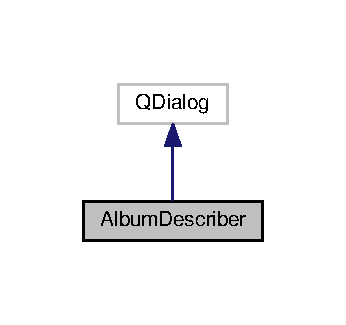
\includegraphics[width=166pt]{class_album_describer__inherit__graph}
\end{center}
\end{figure}


Collaboration diagram for Album\+Describer\+:
\nopagebreak
\begin{figure}[H]
\begin{center}
\leavevmode
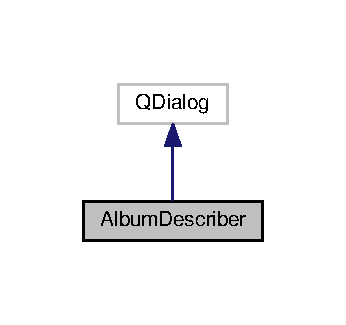
\includegraphics[width=166pt]{class_album_describer__coll__graph}
\end{center}
\end{figure}
\subsection*{Public Member Functions}
\begin{DoxyCompactItemize}
\item 
{\bfseries Album\+Describer} (Q\+Widget $\ast$parent=0)\hypertarget{class_album_describer_ad008c80d667df6a886a326b213d7a97f}{}\label{class_album_describer_ad008c80d667df6a886a326b213d7a97f}

\item 
void {\bfseries update\+Info} (const Album \&album, const Catalog \&catalog)\hypertarget{class_album_describer_af7621a37d31dd0844cb9134ae319c95a}{}\label{class_album_describer_af7621a37d31dd0844cb9134ae319c95a}

\end{DoxyCompactItemize}


The documentation for this class was generated from the following files\+:\begin{DoxyCompactItemize}
\item 
albumdescriber.\+h\item 
albumdescriber.\+cpp\end{DoxyCompactItemize}

\hypertarget{struct_catalog___1_1_album_entity}{}\section{Catalog\+\_\+\+:\+:Album\+Entity Struct Reference}
\label{struct_catalog___1_1_album_entity}\index{Catalog\+\_\+\+::\+Album\+Entity@{Catalog\+\_\+\+::\+Album\+Entity}}
\subsection*{Public Attributes}
\begin{DoxyCompactItemize}
\item 
std\+::string {\bfseries name}\hypertarget{struct_catalog___1_1_album_entity_ac220f4c0491537f157341586f72ac361}{}\label{struct_catalog___1_1_album_entity_ac220f4c0491537f157341586f72ac361}

\item 
std\+::string {\bfseries author}\hypertarget{struct_catalog___1_1_album_entity_a6028eca157f1d9f6fe4f20e07a65f488}{}\label{struct_catalog___1_1_album_entity_a6028eca157f1d9f6fe4f20e07a65f488}

\item 
std\+::string {\bfseries genre}\hypertarget{struct_catalog___1_1_album_entity_a76df9314ecc088b70534547692b64e05}{}\label{struct_catalog___1_1_album_entity_a76df9314ecc088b70534547692b64e05}

\end{DoxyCompactItemize}
\subsection*{Friends}
\begin{DoxyCompactItemize}
\item 
std\+::istream \& {\bfseries operator$>$$>$} (std\+::istream \&stream, \hyperlink{struct_catalog___1_1_album_entity}{Album\+Entity} \&entity)\hypertarget{struct_catalog___1_1_album_entity_a7b4f9b13362aa17219396935907e9337}{}\label{struct_catalog___1_1_album_entity_a7b4f9b13362aa17219396935907e9337}

\end{DoxyCompactItemize}


The documentation for this struct was generated from the following file\+:\begin{DoxyCompactItemize}
\item 
catalog.\+h\end{DoxyCompactItemize}

\hypertarget{struct_album_query__}{}\section{Album\+Query\+\_\+ Struct Reference}
\label{struct_album_query__}\index{Album\+Query\+\_\+@{Album\+Query\+\_\+}}


Inheritance diagram for Album\+Query\+\_\+\+:
\nopagebreak
\begin{figure}[H]
\begin{center}
\leavevmode
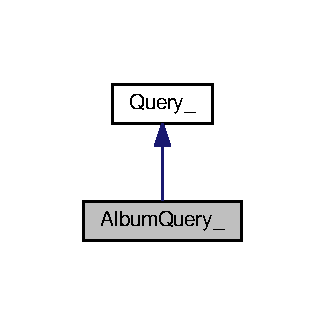
\includegraphics[width=156pt]{struct_album_query____inherit__graph}
\end{center}
\end{figure}


Collaboration diagram for Album\+Query\+\_\+\+:
\nopagebreak
\begin{figure}[H]
\begin{center}
\leavevmode
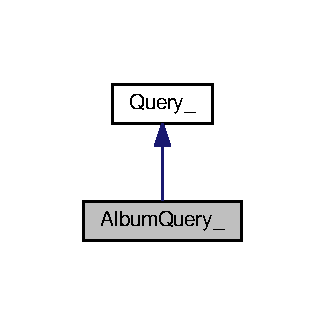
\includegraphics[width=156pt]{struct_album_query____coll__graph}
\end{center}
\end{figure}
\subsection*{Public Member Functions}
\begin{DoxyCompactItemize}
\item 
{\bfseries Album\+Query\+\_\+} (Album album)\hypertarget{struct_album_query___abd744cb06957c0daacc89fb41dd13874}{}\label{struct_album_query___abd744cb06957c0daacc89fb41dd13874}

\item 
bool {\bfseries song\+Matches} (Song song)\hypertarget{struct_album_query___a006936a1e4964df9b1c71227261282d3}{}\label{struct_album_query___a006936a1e4964df9b1c71227261282d3}

\item 
void {\bfseries describe} (std\+::ostream \&stream)\hypertarget{struct_album_query___af3c11ff7248ae1a6c135ace088cb4a24}{}\label{struct_album_query___af3c11ff7248ae1a6c135ace088cb4a24}

\end{DoxyCompactItemize}


The documentation for this struct was generated from the following files\+:\begin{DoxyCompactItemize}
\item 
structures.\+h\item 
structures.\+cpp\end{DoxyCompactItemize}

\hypertarget{struct_author__}{}\section{Author\+\_\+ Struct Reference}
\label{struct_author__}\index{Author\+\_\+@{Author\+\_\+}}
\subsection*{Public Member Functions}
\begin{DoxyCompactItemize}
\item 
void {\bfseries describe} (std\+::ostream \&stream)\hypertarget{struct_author___a9b0dccd6800cdada15353f4099a07793}{}\label{struct_author___a9b0dccd6800cdada15353f4099a07793}

\item 
std\+::string {\bfseries processed\+Name} ()\hypertarget{struct_author___a1e9c33988592236607e0f93226e906e1}{}\label{struct_author___a1e9c33988592236607e0f93226e906e1}

\end{DoxyCompactItemize}
\subsection*{Public Attributes}
\begin{DoxyCompactItemize}
\item 
std\+::string {\bfseries name}\hypertarget{struct_author___a9033f52c9b60dd7abbe05b2975363b5c}{}\label{struct_author___a9033f52c9b60dd7abbe05b2975363b5c}

\item 
std\+::vector$<$ Song $>$ {\bfseries songs}\hypertarget{struct_author___a570029d1a3e6e5532de9ed68d4ee38a4}{}\label{struct_author___a570029d1a3e6e5532de9ed68d4ee38a4}

\item 
std\+::vector$<$ Album $>$ {\bfseries albums}\hypertarget{struct_author___abe54a93ef158880e38afa945d2282f9b}{}\label{struct_author___abe54a93ef158880e38afa945d2282f9b}

\end{DoxyCompactItemize}


The documentation for this struct was generated from the following files\+:\begin{DoxyCompactItemize}
\item 
structures.\+h\item 
structures.\+cpp\end{DoxyCompactItemize}

\hypertarget{class_author_describer}{}\section{Author\+Describer Class Reference}
\label{class_author_describer}\index{Author\+Describer@{Author\+Describer}}


Inheritance diagram for Author\+Describer\+:
\nopagebreak
\begin{figure}[H]
\begin{center}
\leavevmode
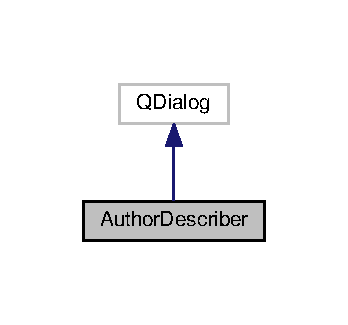
\includegraphics[width=167pt]{class_author_describer__inherit__graph}
\end{center}
\end{figure}


Collaboration diagram for Author\+Describer\+:
\nopagebreak
\begin{figure}[H]
\begin{center}
\leavevmode
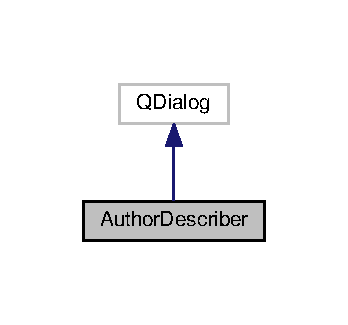
\includegraphics[width=167pt]{class_author_describer__coll__graph}
\end{center}
\end{figure}
\subsection*{Public Member Functions}
\begin{DoxyCompactItemize}
\item 
{\bfseries Author\+Describer} (Q\+Widget $\ast$parent=0)\hypertarget{class_author_describer_ad83461dd5f92afb961598e720eeb58ec}{}\label{class_author_describer_ad83461dd5f92afb961598e720eeb58ec}

\item 
void {\bfseries update\+Info} (const Author \&author, const Catalog \&catalog)\hypertarget{class_author_describer_a862d4e3172a1b5e03fce798ee9db8e9d}{}\label{class_author_describer_a862d4e3172a1b5e03fce798ee9db8e9d}

\end{DoxyCompactItemize}


The documentation for this class was generated from the following files\+:\begin{DoxyCompactItemize}
\item 
authordescriber.\+h\item 
authordescriber.\+cpp\end{DoxyCompactItemize}

\hypertarget{struct_catalog___1_1_author_entity}{}\section{Catalog\+\_\+\+:\+:Author\+Entity Struct Reference}
\label{struct_catalog___1_1_author_entity}\index{Catalog\+\_\+\+::\+Author\+Entity@{Catalog\+\_\+\+::\+Author\+Entity}}
\subsection*{Public Attributes}
\begin{DoxyCompactItemize}
\item 
std\+::string {\bfseries name}\hypertarget{struct_catalog___1_1_author_entity_adb0134112ae346a56aaf02777d3e8fbf}{}\label{struct_catalog___1_1_author_entity_adb0134112ae346a56aaf02777d3e8fbf}

\end{DoxyCompactItemize}
\subsection*{Friends}
\begin{DoxyCompactItemize}
\item 
std\+::istream \& {\bfseries operator$>$$>$} (std\+::istream \&stream, \hyperlink{struct_catalog___1_1_author_entity}{Author\+Entity} \&entity)\hypertarget{struct_catalog___1_1_author_entity_ad6ab10df7184c0f542e5dda14fdce3a0}{}\label{struct_catalog___1_1_author_entity_ad6ab10df7184c0f542e5dda14fdce3a0}

\end{DoxyCompactItemize}


The documentation for this struct was generated from the following file\+:\begin{DoxyCompactItemize}
\item 
catalog.\+h\end{DoxyCompactItemize}

\hypertarget{struct_author_query__}{}\section{Author\+Query\+\_\+ Struct Reference}
\label{struct_author_query__}\index{Author\+Query\+\_\+@{Author\+Query\+\_\+}}


Inheritance diagram for Author\+Query\+\_\+\+:
\nopagebreak
\begin{figure}[H]
\begin{center}
\leavevmode
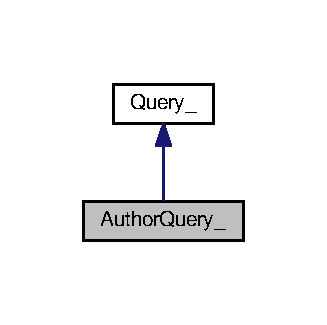
\includegraphics[width=157pt]{struct_author_query____inherit__graph}
\end{center}
\end{figure}


Collaboration diagram for Author\+Query\+\_\+\+:
\nopagebreak
\begin{figure}[H]
\begin{center}
\leavevmode
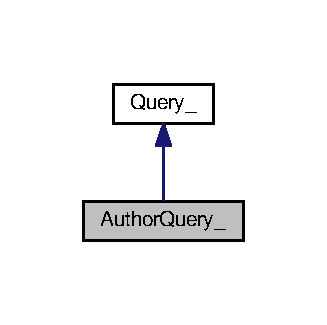
\includegraphics[width=157pt]{struct_author_query____coll__graph}
\end{center}
\end{figure}
\subsection*{Public Member Functions}
\begin{DoxyCompactItemize}
\item 
{\bfseries Author\+Query\+\_\+} (Author author)\hypertarget{struct_author_query___a0279677078b9bb7249517685e3cecd78}{}\label{struct_author_query___a0279677078b9bb7249517685e3cecd78}

\item 
bool {\bfseries song\+Matches} (Song song)\hypertarget{struct_author_query___a1af9eddcf0349da56c8d23ddc7d055e4}{}\label{struct_author_query___a1af9eddcf0349da56c8d23ddc7d055e4}

\item 
void {\bfseries describe} (std\+::ostream \&stream)\hypertarget{struct_author_query___ac336376312ac5ea5c3686237b7c021b9}{}\label{struct_author_query___ac336376312ac5ea5c3686237b7c021b9}

\end{DoxyCompactItemize}


The documentation for this struct was generated from the following files\+:\begin{DoxyCompactItemize}
\item 
structures.\+h\item 
structures.\+cpp\end{DoxyCompactItemize}

\hypertarget{class_catalog__}{}\section{Catalog\+\_\+ Class Reference}
\label{class_catalog__}\index{Catalog\+\_\+@{Catalog\+\_\+}}
\subsection*{Classes}
\begin{DoxyCompactItemize}
\item 
struct \hyperlink{struct_catalog___1_1_album_entity}{Album\+Entity}
\item 
struct \hyperlink{struct_catalog___1_1_author_entity}{Author\+Entity}
\item 
struct \hyperlink{struct_catalog___1_1_genre_entity}{Genre\+Entity}
\item 
struct \hyperlink{struct_catalog___1_1_song_entity}{Song\+Entity}
\end{DoxyCompactItemize}
\subsection*{Public Member Functions}
\begin{DoxyCompactItemize}
\item 
{\bfseries Catalog\+\_\+} (std\+::string file\+Name)\hypertarget{class_catalog___abb39c516b154a11444e1f19afa33bf4e}{}\label{class_catalog___abb39c516b154a11444e1f19afa33bf4e}

\item 
const std\+::vector$<$ Song $>$ \& {\bfseries get\+Songs} ()\hypertarget{class_catalog___a5b4b4d737d7b02c1278c3e3286b7afd5}{}\label{class_catalog___a5b4b4d737d7b02c1278c3e3286b7afd5}

\item 
const std\+::vector$<$ Author $>$ \& {\bfseries get\+Authors} ()\hypertarget{class_catalog___af964934557300f1adc6558e112cc31fa}{}\label{class_catalog___af964934557300f1adc6558e112cc31fa}

\item 
const std\+::vector$<$ Album $>$ \& {\bfseries get\+Albums} ()\hypertarget{class_catalog___a0eba1e6b2ba562cd41e7360af16c2ef5}{}\label{class_catalog___a0eba1e6b2ba562cd41e7360af16c2ef5}

\item 
const std\+::vector$<$ Genre $>$ \& {\bfseries get\+Genres} ()\hypertarget{class_catalog___af8117e2c7d5ddc9d49c4ac707533d565}{}\label{class_catalog___af8117e2c7d5ddc9d49c4ac707533d565}

\item 
const std\+::vector$<$ Song $>$ \& {\bfseries get\+Songs\+By\+Genre} (Genre genre)\hypertarget{class_catalog___aba29098b0061c8d7b83cbe582b6861bf}{}\label{class_catalog___aba29098b0061c8d7b83cbe582b6861bf}

\item 
Author {\bfseries find\+Author} (std\+::string name)\hypertarget{class_catalog___a807b5dc84a686e893a40ebe70b6d6e19}{}\label{class_catalog___a807b5dc84a686e893a40ebe70b6d6e19}

\item 
Genre {\bfseries find\+Genre} (std\+::string name)\hypertarget{class_catalog___a0fee0f49821e1b52cd6c6e737a3f6e6f}{}\label{class_catalog___a0fee0f49821e1b52cd6c6e737a3f6e6f}

\item 
Album {\bfseries find\+Album} (std\+::string name, std\+::string author)\hypertarget{class_catalog___a11d75c63d4fd73a40d3ecd9e88913b72}{}\label{class_catalog___a11d75c63d4fd73a40d3ecd9e88913b72}

\item 
Song {\bfseries find\+Song} (std\+::string name, std\+::string album, std\+::string author)\hypertarget{class_catalog___a4c0fa02c603a172ae2853fd3c7377988}{}\label{class_catalog___a4c0fa02c603a172ae2853fd3c7377988}

\end{DoxyCompactItemize}


The documentation for this class was generated from the following files\+:\begin{DoxyCompactItemize}
\item 
catalog.\+h\item 
catalog.\+cpp\end{DoxyCompactItemize}

\hypertarget{class_catalog_loader}{}\section{Catalog\+Loader Class Reference}
\label{class_catalog_loader}\index{Catalog\+Loader@{Catalog\+Loader}}
\subsection*{Static Public Member Functions}
\begin{DoxyCompactItemize}
\item 
static Catalog {\bfseries load\+Catalog} (std\+::string file\+Name, \hyperlink{class_main_window}{Main\+Window} $\ast$window)\hypertarget{class_catalog_loader_a1dc00fc729be6d5955bca44ecb824dc5}{}\label{class_catalog_loader_a1dc00fc729be6d5955bca44ecb824dc5}

\end{DoxyCompactItemize}


The documentation for this class was generated from the following files\+:\begin{DoxyCompactItemize}
\item 
mainwindow.\+h\item 
mainwindow.\+cpp\end{DoxyCompactItemize}

\hypertarget{struct_end_of_song_event__}{}\section{End\+Of\+Song\+Event\+\_\+ Struct Reference}
\label{struct_end_of_song_event__}\index{End\+Of\+Song\+Event\+\_\+@{End\+Of\+Song\+Event\+\_\+}}


Inheritance diagram for End\+Of\+Song\+Event\+\_\+\+:
\nopagebreak
\begin{figure}[H]
\begin{center}
\leavevmode
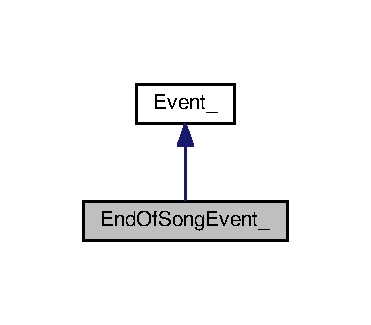
\includegraphics[width=178pt]{struct_end_of_song_event____inherit__graph}
\end{center}
\end{figure}


Collaboration diagram for End\+Of\+Song\+Event\+\_\+\+:
\nopagebreak
\begin{figure}[H]
\begin{center}
\leavevmode
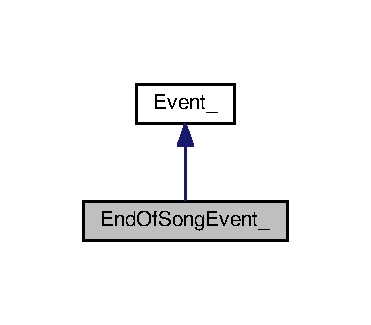
\includegraphics[width=178pt]{struct_end_of_song_event____coll__graph}
\end{center}
\end{figure}
\subsection*{Public Member Functions}
\begin{DoxyCompactItemize}
\item 
{\bfseries End\+Of\+Song\+Event\+\_\+} (int timestamp)\hypertarget{struct_end_of_song_event___a2eb0a3904d21226a08e57f30f46fdeb0}{}\label{struct_end_of_song_event___a2eb0a3904d21226a08e57f30f46fdeb0}

\item 
void {\bfseries polymorphic} ()\hypertarget{struct_end_of_song_event___a99543260e4232f18db1f88e3bc551b5c}{}\label{struct_end_of_song_event___a99543260e4232f18db1f88e3bc551b5c}

\end{DoxyCompactItemize}
\subsection*{Additional Inherited Members}


The documentation for this struct was generated from the following files\+:\begin{DoxyCompactItemize}
\item 
events.\+h\item 
events.\+cpp\end{DoxyCompactItemize}

\hypertarget{struct_event__}{}\section{Event\+\_\+ Struct Reference}
\label{struct_event__}\index{Event\+\_\+@{Event\+\_\+}}


Inheritance diagram for Event\+\_\+\+:
\nopagebreak
\begin{figure}[H]
\begin{center}
\leavevmode
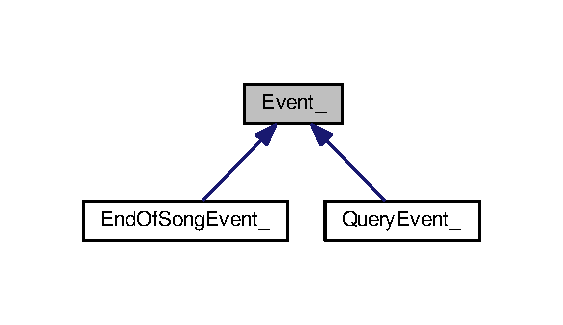
\includegraphics[width=270pt]{struct_event____inherit__graph}
\end{center}
\end{figure}
\subsection*{Public Member Functions}
\begin{DoxyCompactItemize}
\item 
{\bfseries Event\+\_\+} (int timestamp)\hypertarget{struct_event___a480e42487d375d51ffaf8e051ccce162}{}\label{struct_event___a480e42487d375d51ffaf8e051ccce162}

\item 
virtual void {\bfseries polymorphic} ()=0\hypertarget{struct_event___a4330c31a8080eefd1e4824498a492858}{}\label{struct_event___a4330c31a8080eefd1e4824498a492858}

\end{DoxyCompactItemize}
\subsection*{Public Attributes}
\begin{DoxyCompactItemize}
\item 
int {\bfseries timestamp}\hypertarget{struct_event___aa68613c0eac99988b6843cd1bc00cf91}{}\label{struct_event___aa68613c0eac99988b6843cd1bc00cf91}

\end{DoxyCompactItemize}


The documentation for this struct was generated from the following files\+:\begin{DoxyCompactItemize}
\item 
events.\+h\item 
events.\+cpp\end{DoxyCompactItemize}

\hypertarget{struct_radio_program_simulator___1_1_event_comparator}{}\section{Radio\+Program\+Simulator\+\_\+\+:\+:Event\+Comparator Struct Reference}
\label{struct_radio_program_simulator___1_1_event_comparator}\index{Radio\+Program\+Simulator\+\_\+\+::\+Event\+Comparator@{Radio\+Program\+Simulator\+\_\+\+::\+Event\+Comparator}}
\subsection*{Public Member Functions}
\begin{DoxyCompactItemize}
\item 
bool {\bfseries operator()} (const Event \&a, const Event \&b)\hypertarget{struct_radio_program_simulator___1_1_event_comparator_a9a82a5f55ef975881ed775bbba70eeef}{}\label{struct_radio_program_simulator___1_1_event_comparator_a9a82a5f55ef975881ed775bbba70eeef}

\end{DoxyCompactItemize}


The documentation for this struct was generated from the following files\+:\begin{DoxyCompactItemize}
\item 
simulator.\+h\item 
simulator.\+cpp\end{DoxyCompactItemize}

\hypertarget{class_file_utils}{}\section{File\+Utils Class Reference}
\label{class_file_utils}\index{File\+Utils@{File\+Utils}}
\subsection*{Static Public Member Functions}
\begin{DoxyCompactItemize}
\item 
static bool {\bfseries file\+Exists} (std\+::string name)\hypertarget{class_file_utils_a96bf6440f1dd2d7d3a19518e3606f10b}{}\label{class_file_utils_a96bf6440f1dd2d7d3a19518e3606f10b}

\end{DoxyCompactItemize}


The documentation for this class was generated from the following file\+:\begin{DoxyCompactItemize}
\item 
mainwindow.\+h\end{DoxyCompactItemize}

\hypertarget{struct_genre__}{}\section{Genre\+\_\+ Struct Reference}
\label{struct_genre__}\index{Genre\+\_\+@{Genre\+\_\+}}
\subsection*{Public Member Functions}
\begin{DoxyCompactItemize}
\item 
void {\bfseries describe} (std\+::ostream \&stream)\hypertarget{struct_genre___ae7e9b06d07dc4f2704f8e0d474a20edd}{}\label{struct_genre___ae7e9b06d07dc4f2704f8e0d474a20edd}

\item 
std\+::string {\bfseries processed\+Name} ()\hypertarget{struct_genre___aba8a3eaddd8d7fd2d0da9ff7f83801fa}{}\label{struct_genre___aba8a3eaddd8d7fd2d0da9ff7f83801fa}

\end{DoxyCompactItemize}
\subsection*{Public Attributes}
\begin{DoxyCompactItemize}
\item 
std\+::string {\bfseries name}\hypertarget{struct_genre___a8e89d3d7f0c279d298dbfec867b38f14}{}\label{struct_genre___a8e89d3d7f0c279d298dbfec867b38f14}

\end{DoxyCompactItemize}


The documentation for this struct was generated from the following files\+:\begin{DoxyCompactItemize}
\item 
structures.\+h\item 
structures.\+cpp\end{DoxyCompactItemize}

\hypertarget{class_genre_discriber}{}\section{Genre\+Discriber Class Reference}
\label{class_genre_discriber}\index{Genre\+Discriber@{Genre\+Discriber}}


Inheritance diagram for Genre\+Discriber\+:
\nopagebreak
\begin{figure}[H]
\begin{center}
\leavevmode
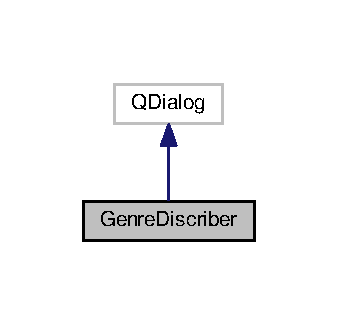
\includegraphics[width=162pt]{class_genre_discriber__inherit__graph}
\end{center}
\end{figure}


Collaboration diagram for Genre\+Discriber\+:
\nopagebreak
\begin{figure}[H]
\begin{center}
\leavevmode
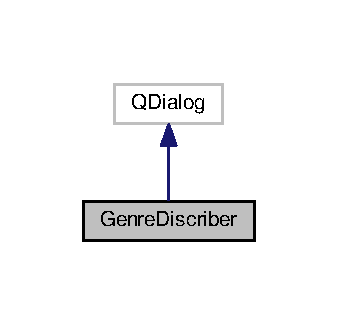
\includegraphics[width=162pt]{class_genre_discriber__coll__graph}
\end{center}
\end{figure}
\subsection*{Public Member Functions}
\begin{DoxyCompactItemize}
\item 
{\bfseries Genre\+Discriber} (Q\+Widget $\ast$parent=0)\hypertarget{class_genre_discriber_aa5b6015fb71401f9b1e99102483b58f7}{}\label{class_genre_discriber_aa5b6015fb71401f9b1e99102483b58f7}

\item 
void {\bfseries update\+Info} (const Genre \&genre, const Catalog \&catalog)\hypertarget{class_genre_discriber_ab1e981c3fec2a53c80ec19ab2fd8f819}{}\label{class_genre_discriber_ab1e981c3fec2a53c80ec19ab2fd8f819}

\end{DoxyCompactItemize}


The documentation for this class was generated from the following files\+:\begin{DoxyCompactItemize}
\item 
genrediscriber.\+h\item 
genrediscriber.\+cpp\end{DoxyCompactItemize}

\hypertarget{struct_catalog___1_1_genre_entity}{}\section{Catalog\+\_\+\+:\+:Genre\+Entity Struct Reference}
\label{struct_catalog___1_1_genre_entity}\index{Catalog\+\_\+\+::\+Genre\+Entity@{Catalog\+\_\+\+::\+Genre\+Entity}}
\subsection*{Public Attributes}
\begin{DoxyCompactItemize}
\item 
std\+::string {\bfseries name}\hypertarget{struct_catalog___1_1_genre_entity_a695790b7c7c4cd43c1e302c35f6aa898}{}\label{struct_catalog___1_1_genre_entity_a695790b7c7c4cd43c1e302c35f6aa898}

\end{DoxyCompactItemize}
\subsection*{Friends}
\begin{DoxyCompactItemize}
\item 
std\+::istream \& {\bfseries operator$>$$>$} (std\+::istream \&stream, \hyperlink{struct_catalog___1_1_genre_entity}{Genre\+Entity} \&entity)\hypertarget{struct_catalog___1_1_genre_entity_a0373ab791f1dcfd45aba717b29b5ef67}{}\label{struct_catalog___1_1_genre_entity_a0373ab791f1dcfd45aba717b29b5ef67}

\end{DoxyCompactItemize}


The documentation for this struct was generated from the following file\+:\begin{DoxyCompactItemize}
\item 
catalog.\+h\end{DoxyCompactItemize}

\hypertarget{class_hit_parad_program__}{}\section{Hit\+Parad\+Program\+\_\+ Class Reference}
\label{class_hit_parad_program__}\index{Hit\+Parad\+Program\+\_\+@{Hit\+Parad\+Program\+\_\+}}


Inheritance diagram for Hit\+Parad\+Program\+\_\+\+:
\nopagebreak
\begin{figure}[H]
\begin{center}
\leavevmode
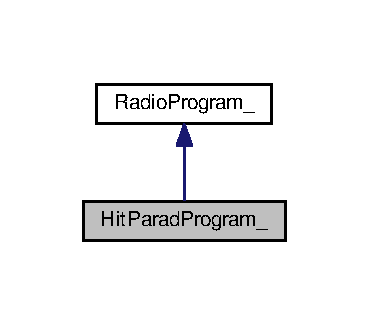
\includegraphics[width=177pt]{class_hit_parad_program____inherit__graph}
\end{center}
\end{figure}


Collaboration diagram for Hit\+Parad\+Program\+\_\+\+:
\nopagebreak
\begin{figure}[H]
\begin{center}
\leavevmode
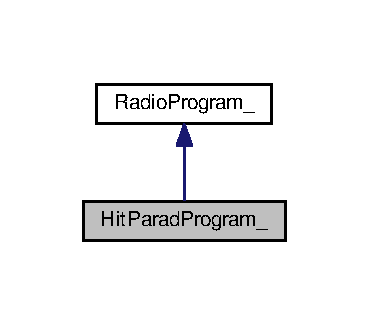
\includegraphics[width=177pt]{class_hit_parad_program____coll__graph}
\end{center}
\end{figure}
\subsection*{Public Member Functions}
\begin{DoxyCompactItemize}
\item 
{\bfseries Hit\+Parad\+Program\+\_\+} (std\+::string name, Genre genre, int start, int duration, Statistics statistics)\hypertarget{class_hit_parad_program___a1097191ce7b288b3dad730dc0b0e8446}{}\label{class_hit_parad_program___a1097191ce7b288b3dad730dc0b0e8446}

\end{DoxyCompactItemize}
\subsection*{Additional Inherited Members}


The documentation for this class was generated from the following files\+:\begin{DoxyCompactItemize}
\item 
radioprogram.\+h\item 
radioprogram.\+cpp\end{DoxyCompactItemize}

\hypertarget{class_hit_parad_program_simulator__}{}\section{Hit\+Parad\+Program\+Simulator\+\_\+ Class Reference}
\label{class_hit_parad_program_simulator__}\index{Hit\+Parad\+Program\+Simulator\+\_\+@{Hit\+Parad\+Program\+Simulator\+\_\+}}


Inheritance diagram for Hit\+Parad\+Program\+Simulator\+\_\+\+:
\nopagebreak
\begin{figure}[H]
\begin{center}
\leavevmode
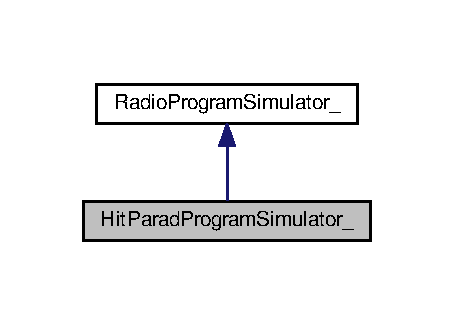
\includegraphics[width=218pt]{class_hit_parad_program_simulator____inherit__graph}
\end{center}
\end{figure}


Collaboration diagram for Hit\+Parad\+Program\+Simulator\+\_\+\+:
\nopagebreak
\begin{figure}[H]
\begin{center}
\leavevmode
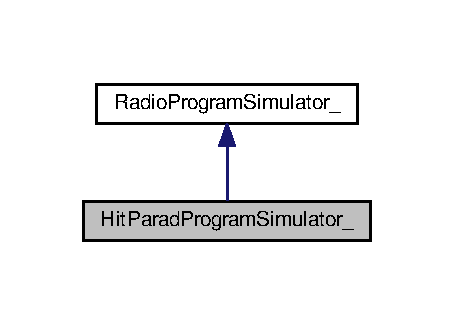
\includegraphics[width=218pt]{class_hit_parad_program_simulator____coll__graph}
\end{center}
\end{figure}
\subsection*{Public Member Functions}
\begin{DoxyCompactItemize}
\item 
{\bfseries Hit\+Parad\+Program\+Simulator\+\_\+} (std\+::string name, Genre genre, int duration, int timestamp, Statistics statistics)\hypertarget{class_hit_parad_program_simulator___a16b7b8d2f2def1484fe6cdc0b6281262}{}\label{class_hit_parad_program_simulator___a16b7b8d2f2def1484fe6cdc0b6281262}

\item 
std\+::vector$<$ Event $>$ {\bfseries build\+Initial\+Events} (Catalog catalog)\hypertarget{class_hit_parad_program_simulator___af8968cffb656c87cbc2df0d15a2d1421}{}\label{class_hit_parad_program_simulator___af8968cffb656c87cbc2df0d15a2d1421}

\item 
void {\bfseries process} (Queue \&events, Event event, Catalog catalog)\hypertarget{class_hit_parad_program_simulator___a9f9186bbcd925f9df0b62eff80621f1b}{}\label{class_hit_parad_program_simulator___a9f9186bbcd925f9df0b62eff80621f1b}

\item 
void {\bfseries end\+Of\+Song\+Event} (Queue \&events, End\+Of\+Song\+Event event, Catalog catalog)\hypertarget{class_hit_parad_program_simulator___a3f4ef80aa460f9b3a636e1c4241631a3}{}\label{class_hit_parad_program_simulator___a3f4ef80aa460f9b3a636e1c4241631a3}

\end{DoxyCompactItemize}
\subsection*{Additional Inherited Members}


The documentation for this class was generated from the following files\+:\begin{DoxyCompactItemize}
\item 
simulator.\+h\item 
simulator.\+cpp\end{DoxyCompactItemize}

\hypertarget{class_main_window}{}\section{Main\+Window Class Reference}
\label{class_main_window}\index{Main\+Window@{Main\+Window}}


Inheritance diagram for Main\+Window\+:
\nopagebreak
\begin{figure}[H]
\begin{center}
\leavevmode
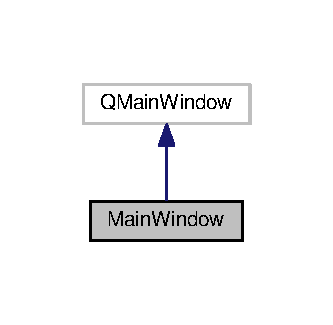
\includegraphics[width=160pt]{class_main_window__inherit__graph}
\end{center}
\end{figure}


Collaboration diagram for Main\+Window\+:
\nopagebreak
\begin{figure}[H]
\begin{center}
\leavevmode
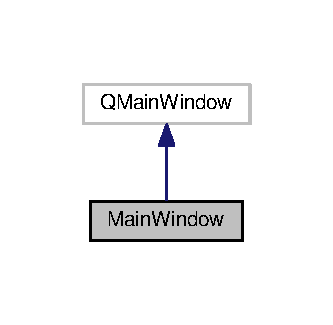
\includegraphics[width=160pt]{class_main_window__coll__graph}
\end{center}
\end{figure}
\subsection*{Public Member Functions}
\begin{DoxyCompactItemize}
\item 
{\bfseries Main\+Window} (Q\+Widget $\ast$parent=0)\hypertarget{class_main_window_a8b244be8b7b7db1b08de2a2acb9409db}{}\label{class_main_window_a8b244be8b7b7db1b08de2a2acb9409db}

\item 
void {\bfseries info\+Box} (std\+::string text)\hypertarget{class_main_window_ae8960cc4d4275957599644c0fe628bca}{}\label{class_main_window_ae8960cc4d4275957599644c0fe628bca}

\end{DoxyCompactItemize}


The documentation for this class was generated from the following files\+:\begin{DoxyCompactItemize}
\item 
mainwindow.\+h\item 
mainwindow.\+cpp\end{DoxyCompactItemize}

\hypertarget{struct_play__}{}\section{Play\+\_\+ Struct Reference}
\label{struct_play__}\index{Play\+\_\+@{Play\+\_\+}}
\subsection*{Public Member Functions}
\begin{DoxyCompactItemize}
\item 
{\bfseries Play\+\_\+} (Song song, int timestamp)\hypertarget{struct_play___a249db3a1ac125aab220ecd109defacc4}{}\label{struct_play___a249db3a1ac125aab220ecd109defacc4}

\end{DoxyCompactItemize}
\subsection*{Public Attributes}
\begin{DoxyCompactItemize}
\item 
Song {\bfseries song}\hypertarget{struct_play___ad288ab8e059a9040e192a00809d7eec4}{}\label{struct_play___ad288ab8e059a9040e192a00809d7eec4}

\item 
int {\bfseries timestamp}\hypertarget{struct_play___a632aa2c9a3ed162e06711577b68bdc3a}{}\label{struct_play___a632aa2c9a3ed162e06711577b68bdc3a}

\end{DoxyCompactItemize}


The documentation for this struct was generated from the following files\+:\begin{DoxyCompactItemize}
\item 
structures.\+h\item 
structures.\+cpp\end{DoxyCompactItemize}

\hypertarget{struct_play_event__}{}\section{Play\+Event\+\_\+ Struct Reference}
\label{struct_play_event__}\index{Play\+Event\+\_\+@{Play\+Event\+\_\+}}


Inheritance diagram for Play\+Event\+\_\+\+:
\nopagebreak
\begin{figure}[H]
\begin{center}
\leavevmode
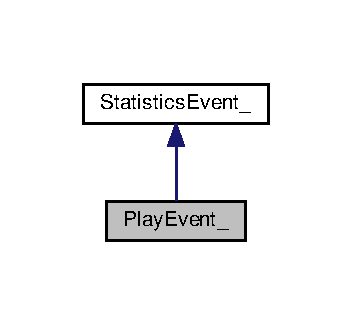
\includegraphics[width=169pt]{struct_play_event____inherit__graph}
\end{center}
\end{figure}


Collaboration diagram for Play\+Event\+\_\+\+:
\nopagebreak
\begin{figure}[H]
\begin{center}
\leavevmode
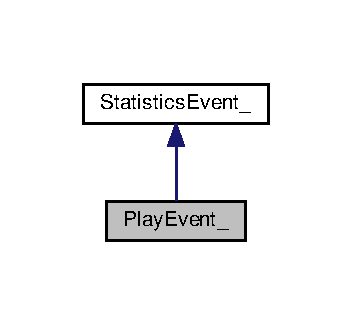
\includegraphics[width=169pt]{struct_play_event____coll__graph}
\end{center}
\end{figure}
\subsection*{Public Member Functions}
\begin{DoxyCompactItemize}
\item 
{\bfseries Play\+Event\+\_\+} (int timestamp, Song song, Radio\+Program program)\hypertarget{struct_play_event___a15a9f81556966a05fff2acf905e48671}{}\label{struct_play_event___a15a9f81556966a05fff2acf905e48671}

\item 
void {\bfseries describe} (std\+::ostream \&stream)\hypertarget{struct_play_event___aedfc9251d901dac44dcba4f70692080a}{}\label{struct_play_event___aedfc9251d901dac44dcba4f70692080a}

\end{DoxyCompactItemize}
\subsection*{Protected Attributes}
\begin{DoxyCompactItemize}
\item 
Song {\bfseries song}\hypertarget{struct_play_event___a7f398c1e252f22dcb6084120f64f627a}{}\label{struct_play_event___a7f398c1e252f22dcb6084120f64f627a}

\item 
Radio\+Program {\bfseries program}\hypertarget{struct_play_event___aaeb553f33dece56c8a0e7caa7ef755b9}{}\label{struct_play_event___aaeb553f33dece56c8a0e7caa7ef755b9}

\end{DoxyCompactItemize}
\subsection*{Additional Inherited Members}


The documentation for this struct was generated from the following files\+:\begin{DoxyCompactItemize}
\item 
events.\+h\item 
events.\+cpp\end{DoxyCompactItemize}

\hypertarget{struct_query__}{}\section{Query\+\_\+ Struct Reference}
\label{struct_query__}\index{Query\+\_\+@{Query\+\_\+}}


Inheritance diagram for Query\+\_\+\+:
\nopagebreak
\begin{figure}[H]
\begin{center}
\leavevmode
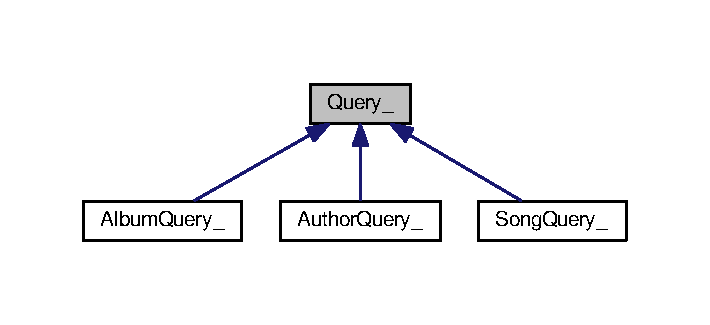
\includegraphics[width=341pt]{struct_query____inherit__graph}
\end{center}
\end{figure}
\subsection*{Public Member Functions}
\begin{DoxyCompactItemize}
\item 
virtual bool {\bfseries song\+Matches} (Song song)=0\hypertarget{struct_query___ae87a04ddd35d72aa7b78acc74049abac}{}\label{struct_query___ae87a04ddd35d72aa7b78acc74049abac}

\item 
virtual void {\bfseries describe} (std\+::ostream \&stream)=0\hypertarget{struct_query___a3b46cf0d317a537e5085f448de42e76b}{}\label{struct_query___a3b46cf0d317a537e5085f448de42e76b}

\item 
{\footnotesize template$<$typename Catalog $>$ }\\std\+::vector$<$ Song $>$ {\bfseries find\+Possible\+Songs} (Catalog catalog)\hypertarget{struct_query___a5f8a9a129903856245b816070aa7264a}{}\label{struct_query___a5f8a9a129903856245b816070aa7264a}

\end{DoxyCompactItemize}


The documentation for this struct was generated from the following files\+:\begin{DoxyCompactItemize}
\item 
structures.\+h\item 
structures.\+cpp\end{DoxyCompactItemize}

\hypertarget{struct_query_event__}{}\section{Query\+Event\+\_\+ Struct Reference}
\label{struct_query_event__}\index{Query\+Event\+\_\+@{Query\+Event\+\_\+}}


Inheritance diagram for Query\+Event\+\_\+\+:
\nopagebreak
\begin{figure}[H]
\begin{center}
\leavevmode
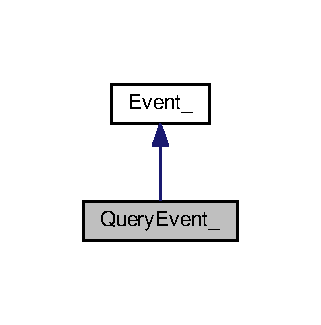
\includegraphics[width=154pt]{struct_query_event____inherit__graph}
\end{center}
\end{figure}


Collaboration diagram for Query\+Event\+\_\+\+:
\nopagebreak
\begin{figure}[H]
\begin{center}
\leavevmode
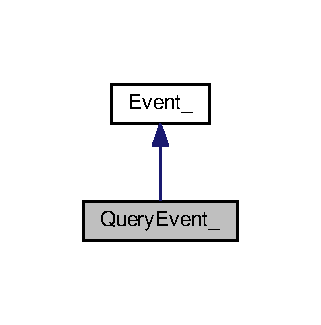
\includegraphics[width=154pt]{struct_query_event____coll__graph}
\end{center}
\end{figure}
\subsection*{Public Member Functions}
\begin{DoxyCompactItemize}
\item 
{\bfseries Query\+Event\+\_\+} (int timestamp, Query query)\hypertarget{struct_query_event___a13e81f98500d5daae31ccb5fb8242fcc}{}\label{struct_query_event___a13e81f98500d5daae31ccb5fb8242fcc}

\item 
void {\bfseries polymorphic} ()\hypertarget{struct_query_event___adf6a63b99179e31b39f74cd96ebac290}{}\label{struct_query_event___adf6a63b99179e31b39f74cd96ebac290}

\end{DoxyCompactItemize}
\subsection*{Public Attributes}
\begin{DoxyCompactItemize}
\item 
Query {\bfseries query}\hypertarget{struct_query_event___abfce144c810ec391ade61dfeebefa3a8}{}\label{struct_query_event___abfce144c810ec391ade61dfeebefa3a8}

\end{DoxyCompactItemize}


The documentation for this struct was generated from the following files\+:\begin{DoxyCompactItemize}
\item 
events.\+h\item 
events.\+cpp\end{DoxyCompactItemize}

\hypertarget{class_radio_program__}{}\section{Radio\+Program\+\_\+ Class Reference}
\label{class_radio_program__}\index{Radio\+Program\+\_\+@{Radio\+Program\+\_\+}}


Inheritance diagram for Radio\+Program\+\_\+\+:
\nopagebreak
\begin{figure}[H]
\begin{center}
\leavevmode
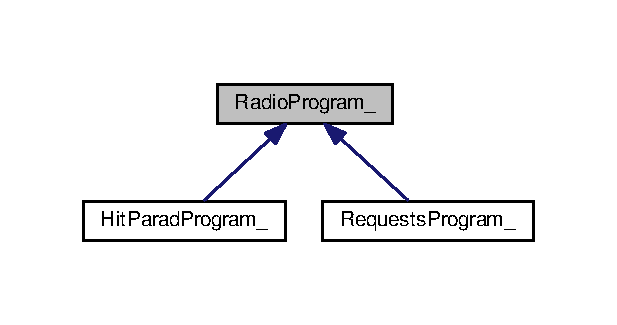
\includegraphics[width=296pt]{class_radio_program____inherit__graph}
\end{center}
\end{figure}
\subsection*{Public Member Functions}
\begin{DoxyCompactItemize}
\item 
{\bfseries Radio\+Program\+\_\+} (std\+::string name, Genre genre, int start, int duration, Statistics statistics)\hypertarget{class_radio_program___adddccea7716c357eea50ba8c325dcd9b}{}\label{class_radio_program___adddccea7716c357eea50ba8c325dcd9b}

\item 
Song {\bfseries pick\+Next\+Song} (Catalog catalog, int timestamp)\hypertarget{class_radio_program___a88bb1b26329c4f217a0192e1601ca13b}{}\label{class_radio_program___a88bb1b26329c4f217a0192e1601ca13b}

\item 
std\+::string {\bfseries get\+Name} ()\hypertarget{class_radio_program___abc521ae542ecdcaca987164f19d94d09}{}\label{class_radio_program___abc521ae542ecdcaca987164f19d94d09}

\end{DoxyCompactItemize}
\subsection*{Protected Member Functions}
\begin{DoxyCompactItemize}
\item 
virtual std\+::map$<$ Song, double $>$ {\bfseries get\+Qualities} (Catalog catalog, int timestamp)=0\hypertarget{class_radio_program___a83a524f556b517f42401e28115e5ccfc}{}\label{class_radio_program___a83a524f556b517f42401e28115e5ccfc}

\item 
virtual void {\bfseries postprocess\+Song} (Song song, int timestamp)=0\hypertarget{class_radio_program___ab862ebc2865ee85472029f4f4dbea3f8}{}\label{class_radio_program___ab862ebc2865ee85472029f4f4dbea3f8}

\end{DoxyCompactItemize}
\subsection*{Protected Attributes}
\begin{DoxyCompactItemize}
\item 
std\+::string {\bfseries name}\hypertarget{class_radio_program___a67daa7da22d48eb820299db912a8bcd9}{}\label{class_radio_program___a67daa7da22d48eb820299db912a8bcd9}

\item 
Genre {\bfseries genre}\hypertarget{class_radio_program___a2d91fcad74fad26085757923f269d9d9}{}\label{class_radio_program___a2d91fcad74fad26085757923f269d9d9}

\item 
int {\bfseries start}\hypertarget{class_radio_program___a496269bda247969a56f0dc7ccb169c03}{}\label{class_radio_program___a496269bda247969a56f0dc7ccb169c03}

\item 
int {\bfseries duration}\hypertarget{class_radio_program___a7fa75a28695c1b571bf529bc4e90cab5}{}\label{class_radio_program___a7fa75a28695c1b571bf529bc4e90cab5}

\item 
Statistics {\bfseries statistics}\hypertarget{class_radio_program___a9978ec8a87c81907594efcea1408501b}{}\label{class_radio_program___a9978ec8a87c81907594efcea1408501b}

\end{DoxyCompactItemize}


The documentation for this class was generated from the following files\+:\begin{DoxyCompactItemize}
\item 
radioprogram.\+h\item 
radioprogram.\+cpp\end{DoxyCompactItemize}

\hypertarget{class_radio_program_simulator__}{}\section{Radio\+Program\+Simulator\+\_\+ Class Reference}
\label{class_radio_program_simulator__}\index{Radio\+Program\+Simulator\+\_\+@{Radio\+Program\+Simulator\+\_\+}}


Inheritance diagram for Radio\+Program\+Simulator\+\_\+\+:
\nopagebreak
\begin{figure}[H]
\begin{center}
\leavevmode
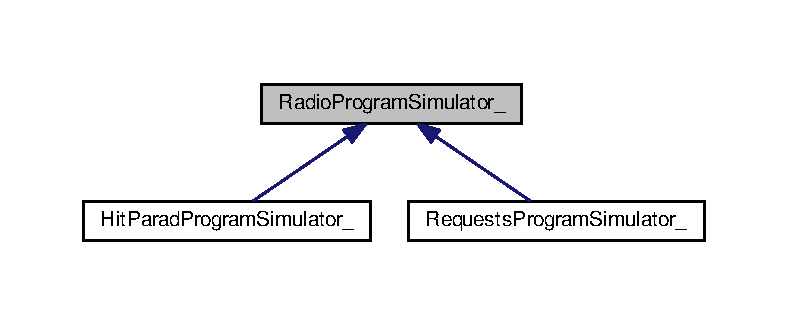
\includegraphics[width=350pt]{class_radio_program_simulator____inherit__graph}
\end{center}
\end{figure}
\subsection*{Classes}
\begin{DoxyCompactItemize}
\item 
struct \hyperlink{struct_radio_program_simulator___1_1_event_comparator}{Event\+Comparator}
\end{DoxyCompactItemize}
\subsection*{Public Types}
\begin{DoxyCompactItemize}
\item 
using {\bfseries Queue} = std\+::set$<$ Event, \hyperlink{struct_radio_program_simulator___1_1_event_comparator}{Event\+Comparator} $>$\hypertarget{class_radio_program_simulator___ac98d8550782603c086c78a7e0cffaa25}{}\label{class_radio_program_simulator___ac98d8550782603c086c78a7e0cffaa25}

\end{DoxyCompactItemize}
\subsection*{Public Member Functions}
\begin{DoxyCompactItemize}
\item 
{\bfseries Radio\+Program\+Simulator\+\_\+} (std\+::string name, Genre genre, int duration, int timestamp, Statistics statistics)\hypertarget{class_radio_program_simulator___a9d26f2e7d90f78c684f50ebd021c05b9}{}\label{class_radio_program_simulator___a9d26f2e7d90f78c684f50ebd021c05b9}

\item 
int {\bfseries simulate} (Catalog catalog)\hypertarget{class_radio_program_simulator___aeb6546c06ad70352ace2b75f42828ec6}{}\label{class_radio_program_simulator___aeb6546c06ad70352ace2b75f42828ec6}

\item 
virtual std\+::vector$<$ Event $>$ {\bfseries build\+Initial\+Events} (Catalog catalog)=0\hypertarget{class_radio_program_simulator___a77382068d8b26c6f4fb481b8f767b728}{}\label{class_radio_program_simulator___a77382068d8b26c6f4fb481b8f767b728}

\item 
virtual void {\bfseries process} (Queue \&events, Event event, Catalog catalog)=0\hypertarget{class_radio_program_simulator___a0b6c6ce7808b0022c744c5aba6ceb0d0}{}\label{class_radio_program_simulator___a0b6c6ce7808b0022c744c5aba6ceb0d0}

\end{DoxyCompactItemize}
\subsection*{Protected Attributes}
\begin{DoxyCompactItemize}
\item 
std\+::string {\bfseries name}\hypertarget{class_radio_program_simulator___af5af6a3c060532ef056afb3716e04007}{}\label{class_radio_program_simulator___af5af6a3c060532ef056afb3716e04007}

\item 
Genre {\bfseries genre}\hypertarget{class_radio_program_simulator___a1da9ac191eaab12a6ae218a0c5301b10}{}\label{class_radio_program_simulator___a1da9ac191eaab12a6ae218a0c5301b10}

\item 
int {\bfseries duration}\hypertarget{class_radio_program_simulator___a075c27dd86b73e53b452ea830de02503}{}\label{class_radio_program_simulator___a075c27dd86b73e53b452ea830de02503}

\item 
int {\bfseries timestamp}\hypertarget{class_radio_program_simulator___a784346e99a688b8a3d2fe028116ad908}{}\label{class_radio_program_simulator___a784346e99a688b8a3d2fe028116ad908}

\item 
Statistics {\bfseries statistics}\hypertarget{class_radio_program_simulator___a4e599f9e0c91ad4299642da77ed75d0a}{}\label{class_radio_program_simulator___a4e599f9e0c91ad4299642da77ed75d0a}

\end{DoxyCompactItemize}


The documentation for this class was generated from the following files\+:\begin{DoxyCompactItemize}
\item 
simulator.\+h\item 
simulator.\+cpp\end{DoxyCompactItemize}

\hypertarget{class_requests_generator}{}\section{Requests\+Generator Class Reference}
\label{class_requests_generator}\index{Requests\+Generator@{Requests\+Generator}}
\subsection*{Public Member Functions}
\begin{DoxyCompactItemize}
\item 
{\bfseries Requests\+Generator} (int timestamp, int duration)\hypertarget{class_requests_generator_acaf8ef7ce01c37b6dec11feefefd6e4b}{}\label{class_requests_generator_acaf8ef7ce01c37b6dec11feefefd6e4b}

\item 
std\+::vector$<$ Event $>$ {\bfseries generate} (Catalog catalog)\hypertarget{class_requests_generator_a4cc136903f250e46ba5d9c381ad90978}{}\label{class_requests_generator_a4cc136903f250e46ba5d9c381ad90978}

\end{DoxyCompactItemize}


The documentation for this class was generated from the following files\+:\begin{DoxyCompactItemize}
\item 
requestsgenerator.\+h\item 
requestsgenerator.\+cpp\end{DoxyCompactItemize}

\hypertarget{class_requests_program__}{}\section{Requests\+Program\+\_\+ Class Reference}
\label{class_requests_program__}\index{Requests\+Program\+\_\+@{Requests\+Program\+\_\+}}


Inheritance diagram for Requests\+Program\+\_\+\+:
\nopagebreak
\begin{figure}[H]
\begin{center}
\leavevmode
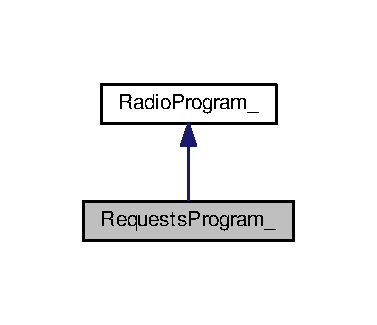
\includegraphics[width=181pt]{class_requests_program____inherit__graph}
\end{center}
\end{figure}


Collaboration diagram for Requests\+Program\+\_\+\+:
\nopagebreak
\begin{figure}[H]
\begin{center}
\leavevmode
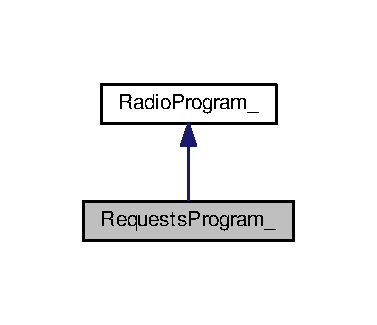
\includegraphics[width=181pt]{class_requests_program____coll__graph}
\end{center}
\end{figure}
\subsection*{Public Member Functions}
\begin{DoxyCompactItemize}
\item 
{\bfseries Requests\+Program\+\_\+} (std\+::string name, Genre genre, int start, int duration, Statistics statistics)\hypertarget{class_requests_program___a59ed61531c124550d37a45520553b123}{}\label{class_requests_program___a59ed61531c124550d37a45520553b123}

\item 
void {\bfseries make\+Query} (int timestamp, Query query)\hypertarget{class_requests_program___a88122fe77f3c341fe2b72d4612e4d7f6}{}\label{class_requests_program___a88122fe77f3c341fe2b72d4612e4d7f6}

\end{DoxyCompactItemize}
\subsection*{Additional Inherited Members}


The documentation for this class was generated from the following files\+:\begin{DoxyCompactItemize}
\item 
radioprogram.\+h\item 
radioprogram.\+cpp\end{DoxyCompactItemize}

\hypertarget{class_requests_program_simulator__}{}\section{Requests\+Program\+Simulator\+\_\+ Class Reference}
\label{class_requests_program_simulator__}\index{Requests\+Program\+Simulator\+\_\+@{Requests\+Program\+Simulator\+\_\+}}


Inheritance diagram for Requests\+Program\+Simulator\+\_\+\+:
\nopagebreak
\begin{figure}[H]
\begin{center}
\leavevmode
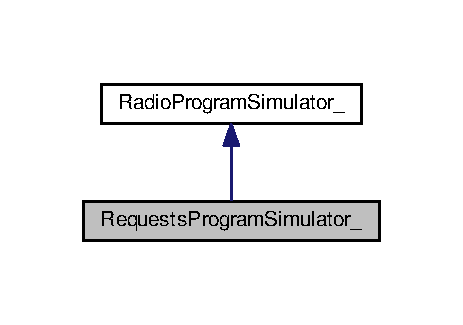
\includegraphics[width=222pt]{class_requests_program_simulator____inherit__graph}
\end{center}
\end{figure}


Collaboration diagram for Requests\+Program\+Simulator\+\_\+\+:
\nopagebreak
\begin{figure}[H]
\begin{center}
\leavevmode
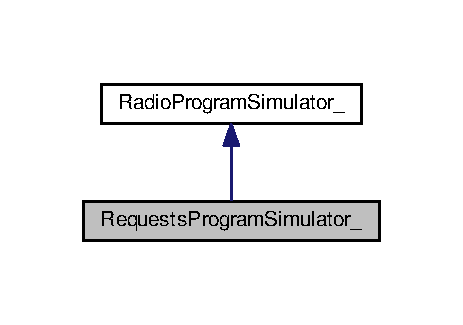
\includegraphics[width=222pt]{class_requests_program_simulator____coll__graph}
\end{center}
\end{figure}
\subsection*{Public Member Functions}
\begin{DoxyCompactItemize}
\item 
{\bfseries Requests\+Program\+Simulator\+\_\+} (std\+::string name, Genre genre, int duration, int timestamp, Statistics statistics)\hypertarget{class_requests_program_simulator___a1f3dd84a16e1d2c4be1de818da52ad02}{}\label{class_requests_program_simulator___a1f3dd84a16e1d2c4be1de818da52ad02}

\item 
std\+::vector$<$ Event $>$ {\bfseries build\+Initial\+Events} (Catalog catalog)\hypertarget{class_requests_program_simulator___a6eb54b7d4e82be9b76e6bbd95e9ad0c0}{}\label{class_requests_program_simulator___a6eb54b7d4e82be9b76e6bbd95e9ad0c0}

\item 
void {\bfseries process} (Queue \&events, Event event, Catalog catalog)\hypertarget{class_requests_program_simulator___a49027fa17e72f83e835a6343e43dd2ec}{}\label{class_requests_program_simulator___a49027fa17e72f83e835a6343e43dd2ec}

\item 
void {\bfseries query} (Queue \&events, Query\+Event event, Catalog catalog)\hypertarget{class_requests_program_simulator___a3b4019d2f26735cf092bc99597df71b7}{}\label{class_requests_program_simulator___a3b4019d2f26735cf092bc99597df71b7}

\item 
void {\bfseries end\+Of\+Song\+Event} (Queue \&events, End\+Of\+Song\+Event event, Catalog catalog)\hypertarget{class_requests_program_simulator___aeaecfe74134600a0982321589481cf1c}{}\label{class_requests_program_simulator___aeaecfe74134600a0982321589481cf1c}

\end{DoxyCompactItemize}
\subsection*{Additional Inherited Members}


The documentation for this class was generated from the following files\+:\begin{DoxyCompactItemize}
\item 
simulator.\+h\item 
simulator.\+cpp\end{DoxyCompactItemize}

\hypertarget{class_royal_manager}{}\section{Royal\+Manager Class Reference}
\label{class_royal_manager}\index{Royal\+Manager@{Royal\+Manager}}
\subsection*{Public Member Functions}
\begin{DoxyCompactItemize}
\item 
{\bfseries Royal\+Manager} (std\+::string catalog\+Path, std\+::string programs\+Path)\hypertarget{class_royal_manager_a4b79671055cc14a68f152defd01724d6}{}\label{class_royal_manager_a4b79671055cc14a68f152defd01724d6}

\item 
Statistics {\bfseries simulate} ()\hypertarget{class_royal_manager_aa114619506c53268470cec99ae3e4280}{}\label{class_royal_manager_aa114619506c53268470cec99ae3e4280}

\end{DoxyCompactItemize}


The documentation for this class was generated from the following files\+:\begin{DoxyCompactItemize}
\item 
royalmanager.\+h\item 
royalmanager.\+cpp\end{DoxyCompactItemize}

\hypertarget{class_simulator__}{}\section{Simulator\+\_\+ Class Reference}
\label{class_simulator__}\index{Simulator\+\_\+@{Simulator\+\_\+}}
\subsection*{Public Member Functions}
\begin{DoxyCompactItemize}
\item 
{\bfseries Simulator\+\_\+} (std\+::string file\+Name)\hypertarget{class_simulator___a14e1afe0c1f6717e4f4eef21419e84ec}{}\label{class_simulator___a14e1afe0c1f6717e4f4eef21419e84ec}

\item 
Statistics {\bfseries simulate} (Catalog catalog)\hypertarget{class_simulator___afb5e8918a23d039cfc31ab8abc921498}{}\label{class_simulator___afb5e8918a23d039cfc31ab8abc921498}

\end{DoxyCompactItemize}
\subsection*{Public Attributes}
\begin{DoxyCompactItemize}
\item 
std\+::vector$<$ std\+::tuple$<$ std\+::string, std\+::string, std\+::string, int $>$ $>$ {\bfseries entities}\hypertarget{class_simulator___ab8ffd354ca15eb30cd1f33ddfa1933c8}{}\label{class_simulator___ab8ffd354ca15eb30cd1f33ddfa1933c8}

\end{DoxyCompactItemize}


The documentation for this class was generated from the following files\+:\begin{DoxyCompactItemize}
\item 
simulator.\+h\item 
simulator.\+cpp\end{DoxyCompactItemize}

\hypertarget{struct_song__}{}\section{Song\+\_\+ Struct Reference}
\label{struct_song__}\index{Song\+\_\+@{Song\+\_\+}}
\subsection*{Public Member Functions}
\begin{DoxyCompactItemize}
\item 
void {\bfseries describe} (std\+::ostream \&stream)\hypertarget{struct_song___a8e10f0e16d2a33ba48b9955af12f9e1b}{}\label{struct_song___a8e10f0e16d2a33ba48b9955af12f9e1b}

\item 
std\+::string {\bfseries processed\+Name} ()\hypertarget{struct_song___a54a55b6d0992acb3d837a4ab3dd39e3a}{}\label{struct_song___a54a55b6d0992acb3d837a4ab3dd39e3a}

\item 
std\+::string {\bfseries processed\+Description} ()\hypertarget{struct_song___a8590717ee470e51084b5962ab31132ed}{}\label{struct_song___a8590717ee470e51084b5962ab31132ed}

\end{DoxyCompactItemize}
\subsection*{Public Attributes}
\begin{DoxyCompactItemize}
\item 
Author {\bfseries author}\hypertarget{struct_song___a22b6bac1012407ac1c4466a92dcc5a02}{}\label{struct_song___a22b6bac1012407ac1c4466a92dcc5a02}

\item 
Album {\bfseries album}\hypertarget{struct_song___a3f2e9d863061c065520c215491272f5e}{}\label{struct_song___a3f2e9d863061c065520c215491272f5e}

\item 
std\+::string {\bfseries name}\hypertarget{struct_song___a741b8c59b73c0569f7596f564d96ce92}{}\label{struct_song___a741b8c59b73c0569f7596f564d96ce92}

\item 
int {\bfseries duration}\hypertarget{struct_song___aa447371b3e9bd8d275d98e152d2e1613}{}\label{struct_song___aa447371b3e9bd8d275d98e152d2e1613}

\item 
Genre {\bfseries genre}\hypertarget{struct_song___a9bc80c8856f1e39234e61517d989a014}{}\label{struct_song___a9bc80c8856f1e39234e61517d989a014}

\end{DoxyCompactItemize}


The documentation for this struct was generated from the following files\+:\begin{DoxyCompactItemize}
\item 
structures.\+h\item 
structures.\+cpp\end{DoxyCompactItemize}

\hypertarget{class_song_describer}{}\section{Song\+Describer Class Reference}
\label{class_song_describer}\index{Song\+Describer@{Song\+Describer}}


Inheritance diagram for Song\+Describer\+:
\nopagebreak
\begin{figure}[H]
\begin{center}
\leavevmode
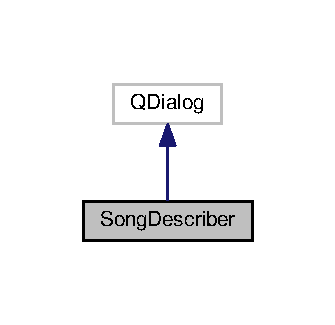
\includegraphics[width=161pt]{class_song_describer__inherit__graph}
\end{center}
\end{figure}


Collaboration diagram for Song\+Describer\+:
\nopagebreak
\begin{figure}[H]
\begin{center}
\leavevmode
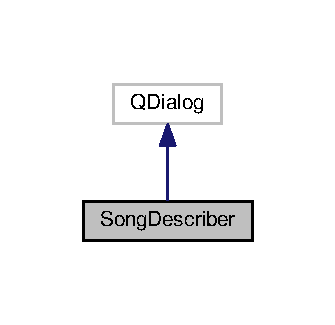
\includegraphics[width=161pt]{class_song_describer__coll__graph}
\end{center}
\end{figure}
\subsection*{Public Member Functions}
\begin{DoxyCompactItemize}
\item 
{\bfseries Song\+Describer} (Q\+Widget $\ast$parent=0)\hypertarget{class_song_describer_a9350e24e4c32132e1075e88f3ff45466}{}\label{class_song_describer_a9350e24e4c32132e1075e88f3ff45466}

\item 
void {\bfseries update\+Info} (const Song \&song, const Catalog \&catalog)\hypertarget{class_song_describer_ad21d4bf2bd9eb5b75f1f9162c37185d8}{}\label{class_song_describer_ad21d4bf2bd9eb5b75f1f9162c37185d8}

\end{DoxyCompactItemize}


The documentation for this class was generated from the following files\+:\begin{DoxyCompactItemize}
\item 
songdescriber.\+h\item 
songdescriber.\+cpp\end{DoxyCompactItemize}

\hypertarget{struct_catalog___1_1_song_entity}{}\section{Catalog\+\_\+\+:\+:Song\+Entity Struct Reference}
\label{struct_catalog___1_1_song_entity}\index{Catalog\+\_\+\+::\+Song\+Entity@{Catalog\+\_\+\+::\+Song\+Entity}}
\subsection*{Public Attributes}
\begin{DoxyCompactItemize}
\item 
std\+::string {\bfseries name}\hypertarget{struct_catalog___1_1_song_entity_a37663964ded7eeeb3509b662979ccd14}{}\label{struct_catalog___1_1_song_entity_a37663964ded7eeeb3509b662979ccd14}

\item 
std\+::string {\bfseries album}\hypertarget{struct_catalog___1_1_song_entity_a65909708e08707a2fc3b3aa95ef4c2dd}{}\label{struct_catalog___1_1_song_entity_a65909708e08707a2fc3b3aa95ef4c2dd}

\item 
std\+::string {\bfseries author}\hypertarget{struct_catalog___1_1_song_entity_a7e7b2bd61852f0f1eed33ac066271e7a}{}\label{struct_catalog___1_1_song_entity_a7e7b2bd61852f0f1eed33ac066271e7a}

\item 
int {\bfseries duration}\hypertarget{struct_catalog___1_1_song_entity_a3e4c02e257540b6ba7c064b6b05aac5a}{}\label{struct_catalog___1_1_song_entity_a3e4c02e257540b6ba7c064b6b05aac5a}

\end{DoxyCompactItemize}
\subsection*{Friends}
\begin{DoxyCompactItemize}
\item 
std\+::istream \& {\bfseries operator$>$$>$} (std\+::istream \&stream, \hyperlink{struct_catalog___1_1_song_entity}{Song\+Entity} \&entity)\hypertarget{struct_catalog___1_1_song_entity_ae082a65fcb118db86a76b5bc171cf01f}{}\label{struct_catalog___1_1_song_entity_ae082a65fcb118db86a76b5bc171cf01f}

\end{DoxyCompactItemize}


The documentation for this struct was generated from the following file\+:\begin{DoxyCompactItemize}
\item 
catalog.\+h\end{DoxyCompactItemize}

\hypertarget{struct_song_query__}{}\section{Song\+Query\+\_\+ Struct Reference}
\label{struct_song_query__}\index{Song\+Query\+\_\+@{Song\+Query\+\_\+}}


Inheritance diagram for Song\+Query\+\_\+\+:
\nopagebreak
\begin{figure}[H]
\begin{center}
\leavevmode
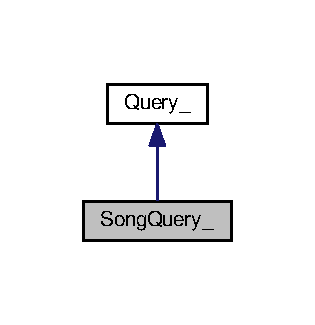
\includegraphics[width=151pt]{struct_song_query____inherit__graph}
\end{center}
\end{figure}


Collaboration diagram for Song\+Query\+\_\+\+:
\nopagebreak
\begin{figure}[H]
\begin{center}
\leavevmode
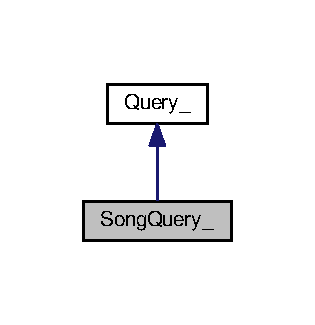
\includegraphics[width=151pt]{struct_song_query____coll__graph}
\end{center}
\end{figure}
\subsection*{Public Member Functions}
\begin{DoxyCompactItemize}
\item 
{\bfseries Song\+Query\+\_\+} (Song song)\hypertarget{struct_song_query___a37355624abafe27a440a803eabefc280}{}\label{struct_song_query___a37355624abafe27a440a803eabefc280}

\item 
bool {\bfseries song\+Matches} (Song song)\hypertarget{struct_song_query___a368afb7c4b4ef2fc2e80be780486f014}{}\label{struct_song_query___a368afb7c4b4ef2fc2e80be780486f014}

\item 
void {\bfseries describe} (std\+::ostream \&stream)\hypertarget{struct_song_query___a75720a128cebaa5affda9fef1cac04b2}{}\label{struct_song_query___a75720a128cebaa5affda9fef1cac04b2}

\end{DoxyCompactItemize}


The documentation for this struct was generated from the following files\+:\begin{DoxyCompactItemize}
\item 
structures.\+h\item 
structures.\+cpp\end{DoxyCompactItemize}

\hypertarget{class_statistics__}{}\section{Statistics\+\_\+ Class Reference}
\label{class_statistics__}\index{Statistics\+\_\+@{Statistics\+\_\+}}
\subsection*{Public Member Functions}
\begin{DoxyCompactItemize}
\item 
const std\+::vector$<$ Play $>$ \& {\bfseries get\+Plays} ()\hypertarget{class_statistics___accdf5145c6545c7e7d3e46e2fb177045}{}\label{class_statistics___accdf5145c6545c7e7d3e46e2fb177045}

\item 
int {\bfseries get\+Song\+Requests\+Count} (Song song)\hypertarget{class_statistics___a50c6d8e2f8bae1d221c0f5479523c789}{}\label{class_statistics___a50c6d8e2f8bae1d221c0f5479523c789}

\item 
void {\bfseries add\+Play} (Radio\+Program program, Song song, int timestamp)\hypertarget{class_statistics___a0003b5b1fe6d1989d67757f15b5a97f5}{}\label{class_statistics___a0003b5b1fe6d1989d67757f15b5a97f5}

\item 
void {\bfseries add\+Query} (Radio\+Program program, Query query, int timestamp)\hypertarget{class_statistics___a1cde5f647ea1d453a76aa51741d4ff4c}{}\label{class_statistics___a1cde5f647ea1d453a76aa51741d4ff4c}

\item 
void {\bfseries print\+Stats} ()\hypertarget{class_statistics___a7b5b41ea831dc710cb6e8b1fade96bee}{}\label{class_statistics___a7b5b41ea831dc710cb6e8b1fade96bee}

\item 
const std\+::vector$<$ Statistics\+Event $>$ \& {\bfseries get\+Events} ()\hypertarget{class_statistics___a7b3b46f2a805db69f0840800e7f1436f}{}\label{class_statistics___a7b3b46f2a805db69f0840800e7f1436f}

\end{DoxyCompactItemize}


The documentation for this class was generated from the following files\+:\begin{DoxyCompactItemize}
\item 
statistics.\+h\item 
statistics.\+cpp\end{DoxyCompactItemize}

\hypertarget{struct_statistics_event__}{}\section{Statistics\+Event\+\_\+ Struct Reference}
\label{struct_statistics_event__}\index{Statistics\+Event\+\_\+@{Statistics\+Event\+\_\+}}


Inheritance diagram for Statistics\+Event\+\_\+\+:
\nopagebreak
\begin{figure}[H]
\begin{center}
\leavevmode
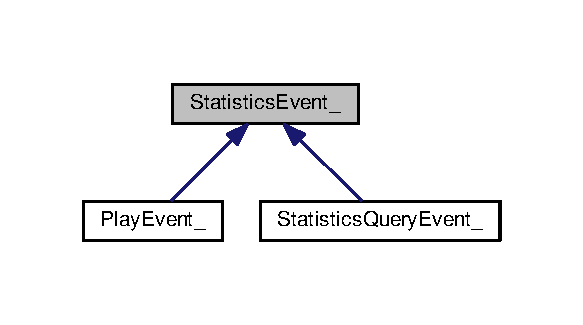
\includegraphics[width=280pt]{struct_statistics_event____inherit__graph}
\end{center}
\end{figure}
\subsection*{Public Member Functions}
\begin{DoxyCompactItemize}
\item 
{\bfseries Statistics\+Event\+\_\+} (int timestamp)\hypertarget{struct_statistics_event___ad2129dfed5eec03929d58755df7e9ec6}{}\label{struct_statistics_event___ad2129dfed5eec03929d58755df7e9ec6}

\item 
virtual void {\bfseries describe} (std\+::ostream \&stream)=0\hypertarget{struct_statistics_event___a2db4e4f8deeaddcea32bac29b38c5866}{}\label{struct_statistics_event___a2db4e4f8deeaddcea32bac29b38c5866}

\end{DoxyCompactItemize}
\subsection*{Public Attributes}
\begin{DoxyCompactItemize}
\item 
int {\bfseries timestamp}\hypertarget{struct_statistics_event___afb83303a81af3c73cbd418a2a5eb5119}{}\label{struct_statistics_event___afb83303a81af3c73cbd418a2a5eb5119}

\end{DoxyCompactItemize}


The documentation for this struct was generated from the following files\+:\begin{DoxyCompactItemize}
\item 
events.\+h\item 
events.\+cpp\end{DoxyCompactItemize}

\hypertarget{struct_statistics_query_event__}{}\section{Statistics\+Query\+Event\+\_\+ Struct Reference}
\label{struct_statistics_query_event__}\index{Statistics\+Query\+Event\+\_\+@{Statistics\+Query\+Event\+\_\+}}


Inheritance diagram for Statistics\+Query\+Event\+\_\+\+:
\nopagebreak
\begin{figure}[H]
\begin{center}
\leavevmode
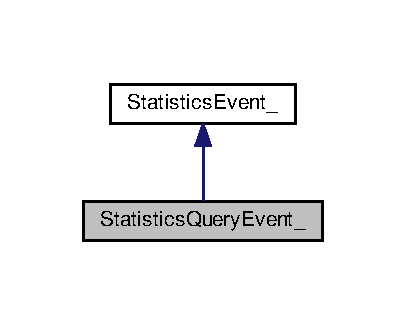
\includegraphics[width=195pt]{struct_statistics_query_event____inherit__graph}
\end{center}
\end{figure}


Collaboration diagram for Statistics\+Query\+Event\+\_\+\+:
\nopagebreak
\begin{figure}[H]
\begin{center}
\leavevmode
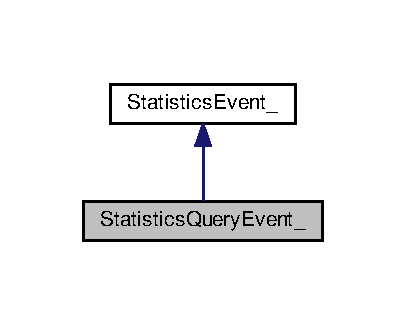
\includegraphics[width=195pt]{struct_statistics_query_event____coll__graph}
\end{center}
\end{figure}
\subsection*{Public Member Functions}
\begin{DoxyCompactItemize}
\item 
{\bfseries Statistics\+Query\+Event\+\_\+} (int timestamp, Query query, Radio\+Program program)\hypertarget{struct_statistics_query_event___acbf94d21664dcdaa682c3b91e14254cd}{}\label{struct_statistics_query_event___acbf94d21664dcdaa682c3b91e14254cd}

\item 
void {\bfseries describe} (std\+::ostream \&stream)\hypertarget{struct_statistics_query_event___a1301f4046157f43d337d80e195a10e42}{}\label{struct_statistics_query_event___a1301f4046157f43d337d80e195a10e42}

\end{DoxyCompactItemize}
\subsection*{Protected Attributes}
\begin{DoxyCompactItemize}
\item 
Query {\bfseries query}\hypertarget{struct_statistics_query_event___a8051ba260ffcdf4f9c4241de790a3ed9}{}\label{struct_statistics_query_event___a8051ba260ffcdf4f9c4241de790a3ed9}

\item 
Radio\+Program {\bfseries program}\hypertarget{struct_statistics_query_event___ad803163d127b9b09d79491da78cd7425}{}\label{struct_statistics_query_event___ad803163d127b9b09d79491da78cd7425}

\end{DoxyCompactItemize}
\subsection*{Additional Inherited Members}


The documentation for this struct was generated from the following files\+:\begin{DoxyCompactItemize}
\item 
events.\+h\item 
events.\+cpp\end{DoxyCompactItemize}

\hypertarget{class_storage_form}{}\section{Storage\+Form Class Reference}
\label{class_storage_form}\index{Storage\+Form@{Storage\+Form}}


Inheritance diagram for Storage\+Form\+:
\nopagebreak
\begin{figure}[H]
\begin{center}
\leavevmode
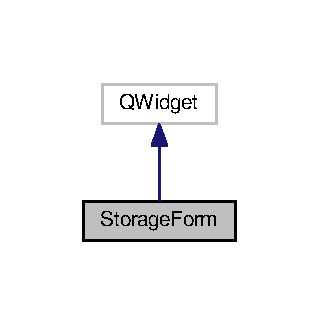
\includegraphics[width=153pt]{class_storage_form__inherit__graph}
\end{center}
\end{figure}


Collaboration diagram for Storage\+Form\+:
\nopagebreak
\begin{figure}[H]
\begin{center}
\leavevmode
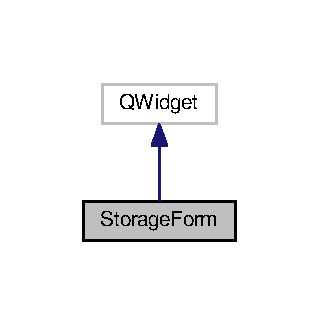
\includegraphics[width=153pt]{class_storage_form__coll__graph}
\end{center}
\end{figure}
\subsection*{Public Member Functions}
\begin{DoxyCompactItemize}
\item 
{\bfseries Storage\+Form} (Q\+Widget $\ast$parent=0)\hypertarget{class_storage_form_a6a989c31e8fa6e48c6e1bf155956ac4c}{}\label{class_storage_form_a6a989c31e8fa6e48c6e1bf155956ac4c}

\end{DoxyCompactItemize}


The documentation for this class was generated from the following files\+:\begin{DoxyCompactItemize}
\item 
storageform.\+h\item 
storageform.\+cpp\end{DoxyCompactItemize}

\hypertarget{class_timetable_editor_form}{}\section{Timetable\+Editor\+Form Class Reference}
\label{class_timetable_editor_form}\index{Timetable\+Editor\+Form@{Timetable\+Editor\+Form}}


Inheritance diagram for Timetable\+Editor\+Form\+:
\nopagebreak
\begin{figure}[H]
\begin{center}
\leavevmode
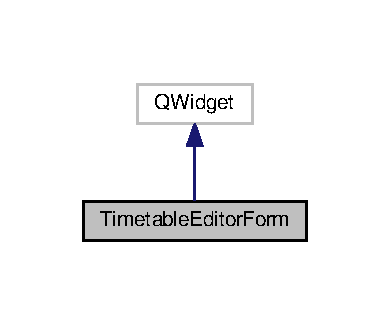
\includegraphics[width=187pt]{class_timetable_editor_form__inherit__graph}
\end{center}
\end{figure}


Collaboration diagram for Timetable\+Editor\+Form\+:
\nopagebreak
\begin{figure}[H]
\begin{center}
\leavevmode
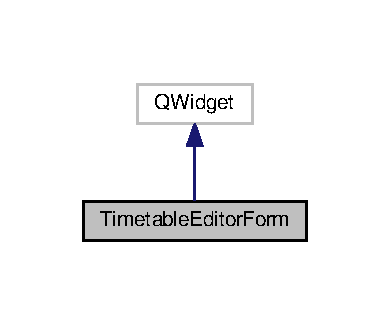
\includegraphics[width=187pt]{class_timetable_editor_form__coll__graph}
\end{center}
\end{figure}
\subsection*{Public Member Functions}
\begin{DoxyCompactItemize}
\item 
{\bfseries Timetable\+Editor\+Form} (Q\+Widget $\ast$parent=0)\hypertarget{class_timetable_editor_form_ac71380513c6d189dee464071970ff304}{}\label{class_timetable_editor_form_ac71380513c6d189dee464071970ff304}

\item 
void {\bfseries accept\+Timetable} (Simulator simulator, Catalog catalog)\hypertarget{class_timetable_editor_form_aa61d64a28d26bf2f3651f014abf83438}{}\label{class_timetable_editor_form_aa61d64a28d26bf2f3651f014abf83438}

\item 
void {\bfseries reshow\+Timetable} ()\hypertarget{class_timetable_editor_form_a813efeb779a096d26295dc143af4e899}{}\label{class_timetable_editor_form_a813efeb779a096d26295dc143af4e899}

\end{DoxyCompactItemize}


The documentation for this class was generated from the following files\+:\begin{DoxyCompactItemize}
\item 
timetableeditorform.\+h\item 
timetableeditorform.\+cpp\end{DoxyCompactItemize}

\hypertarget{class_timetable_loader}{}\section{Timetable\+Loader Class Reference}
\label{class_timetable_loader}\index{Timetable\+Loader@{Timetable\+Loader}}
\subsection*{Static Public Member Functions}
\begin{DoxyCompactItemize}
\item 
static Simulator {\bfseries load\+Timetable} (std\+::string file\+Name, \hyperlink{class_main_window}{Main\+Window} $\ast$window)\hypertarget{class_timetable_loader_a0767ca0adc613d13bcd031336c917950}{}\label{class_timetable_loader_a0767ca0adc613d13bcd031336c917950}

\end{DoxyCompactItemize}


The documentation for this class was generated from the following files\+:\begin{DoxyCompactItemize}
\item 
mainwindow.\+h\item 
mainwindow.\+cpp\end{DoxyCompactItemize}

%--- End generated contents ---

% Index
\backmatter
\newpage
\phantomsection
\clearemptydoublepage
\addcontentsline{toc}{chapter}{Index}
\printindex

\end{document}
